\documentclass[a4paper]{jsarticle}
  \usepackage[T1]{fontenc}
\usepackage{lmodern}
%
\usepackage{amsmath}
\usepackage{amssymb}
\usepackage{bm}
\usepackage[dvipdfmx]{xcolor}
\usepackage[dvipdfmx]{graphicx}
\usepackage{tikz}
\usetikzlibrary{patterns}
\usepackage{ascmac}
\usepackage{multirow}
%
\usepackage{gfncmd}
\usetimessetMatrix
\makeparenwidthresized
%
\usepackage{gfnlf}
\usepackage{gfndecox}
\usepackage{gfndecox-std1}
\usepackage{gfncls}
\setsectiontheme{strongline}
%
\setlength{\parskip}{1em}

  \usepackage{style}
%
  \title{線型数理要論}
  \author{\texttt{@bd\string_gfngfn}}
\begin{document}
\maketitle
%
\setcounter{section}{-1}%(nonsemantic)
\section{はじめに}
  \subsection{概要}
    \plainpar{}{
      この文書では,あまり基底のとり方や線型写像といった一般の議論を意識せず,
      行列を単に「体 $K$ の元が $m \times n$ に並んだもの」として捉えてその性質を見ていく方針をとる.
    }
  \subsection{基本的定義}
    \defpar{}{
      非負整数を\newword{自然数}といい,自然数全体からなる集合を $\setN$,また正整数全体からなる集合を $\setNpos$ と書く.
      自然数 $n \in \setN$ に対し,
      $\Natleq{n} \defeq \setprnsep{k \in \setNpos}{k \leq n}$ とする.
    }
    \defpar{行列に関する記法}{
      体 $\seqprn{K, +, \cdot; 0, 1, \paren{\dummysign}^{-1}}$ の元を並べた
      $m \times n$ 行列全体からなる集合を $\setMatrix{m}{n}{K}$ と書く.
      行列 $A \in \setMatrix{m}{n}{K}$ の $\seqprn{i, j}$ 成分を $A_{i j}$,第 $j$ 列を $\colvec{A}{j}$ と書く.
      $A \in \setMatrix{m}{n}{K}$ に対し,各 $j \in \Natleq{n}$ に於いて
      \begin{align*}
        \colvec{B}{j} &\defeq
          \begin{cases}
            \vecb         &\caseif{j = k}\\
            \colvec{A}{j} &\caseow
          \end{cases}
      \end{align*}
      で定められる行列 $B \in \setMatrix{m}{n}{K}$,すなわち“$A$ の第 $k$ 列をベクトル $\vecb$ で上書きした行列”を
      $\coloverwrite{A}{k}{\vecb}$ と書く.
      また $A \in \setMatrix{m}{n}{K}$ と $I \subseteq \Natleq{m}$ に対して
      “$A$ のうち $I$ に属する行番号だけ取り出した $\card{I} \times n$ 行列”を $\rowsubmatrix{A}{I}$ と書き,
      $J \subseteq \Natleq{n}$ に対して
      “$A$ のうち $J$ に属する列番号だけ取り出した $m \times \card{J}$ 行列”を $\colsubmatrix{A}{J}$ と書く.
    }
\section{行列と行列式}
  \subsection{ブロック行列}
    \thmpar[thm:det-mult-homomorphism]{行列式演算と積の準同型性}{
      正方行列 $A, B \in \setMatrix{n}{n}{K}$ に対して
      \begin{align*}
        \det \paren{A B} = \det A \cdot \det B
      \end{align*}
      が成り立つ.
    }
    \thmpar[thm:block-det-ignore-upper-right]{ブロック零行列による行列式の簡単化}{
      正方行列
      $\DS
        M =
        \text{\raisebox{0.75em}{$\DS
          \begin{array}{@{}r@{}r@{}c@{}c@{}l@{}}
            &
            & \tikz \draw[latex-latex] (0, 0) -- (2em, 0) node[midway, above] {$m$};
            & \tikz \draw[latex-latex] (0, 0) -- (2em, 0) node[midway, above] {$n$};
            &
          \\
            m
            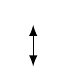
\begin{tikzpicture}
              \path[use as bounding box] (-0.2em, 0) -- (0, 0) -- (0, 1em) -- (-0.2em, 1em) -- cycle;
              \draw[latex-latex] (0, -0.4em) -- (0, 1.1em);
            \end{tikzpicture} &
            \multirow{2}{*}{$\DS \left(\rule[-1.25em]{0pt}{3em}\right.$}
              & \multicolumn{1}{c|}{A}
              & 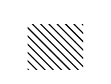
\begin{tikzpicture}
                  \path[use as bounding box] (-1em, 0) rectangle (1em, 1em);
                  \fill[pattern=north west lines] (-1em, -0.5em) rectangle (1em, 1.1em);
                \end{tikzpicture} &
            \multirow{2}{*}{$\DS \left.\rule[-1.25em]{0pt}{3em}\right)$}
          \\\cline{3-4}
            n
            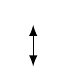
\begin{tikzpicture}
              \path[use as bounding box] (-0.2em, 0) -- (0, 0) -- (0, 1em) -- (-0.2em, 1em) -- cycle;
              \draw[latex-latex] (0, -0.4em) -- (0, 1.1em);
            \end{tikzpicture} &
            & \multicolumn{1}{c|}{O} & \multicolumn{1}{c}{B} &
          \end{array}
        $}}
        \in \setMatrix{\paren{m + n}}{\paren{m + n}}{K}
      $
      に対して
      \begin{align*}
        \det M = \det A \cdot \det B
      \end{align*}
      が成り立つ.
    }
    \thmpar[thm:block-fundamental]{}{
      正方行列
      $\DS
        M =
        \text{\raisebox{0.75em}{$\DS
          \begin{array}{@{}r@{}r@{}c@{}c@{}l@{}}
            &
            & \tikz \draw[latex-latex] (0, 0) -- (2em, 0) node[midway, above] {$m$};
            & \tikz \draw[latex-latex] (0, 0) -- (2em, 0) node[midway, above] {$n$};
            &
          \\
            m
            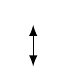
\begin{tikzpicture}
              \path[use as bounding box] (-0.2em, 0) -- (0, 0) -- (0, 1em) -- (-0.2em, 1em) -- cycle;
              \draw[latex-latex] (0, -0.4em) -- (0, 1.1em);
            \end{tikzpicture} &
            \multirow{2}{*}{$\DS \left(\rule[-1.25em]{0pt}{3em}\right.$}
              & \multicolumn{1}{c|}{A} & \multicolumn{1}{c}{B} &
            \multirow{2}{*}{$\DS \left.\rule[-1.25em]{0pt}{3em}\right)$}
          \\\cline{3-4}
            n
            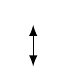
\begin{tikzpicture}
              \path[use as bounding box] (-0.2em, 0) -- (0, 0) -- (0, 1em) -- (-0.2em, 1em) -- cycle;
              \draw[latex-latex] (0, -0.4em) -- (0, 1.1em);
            \end{tikzpicture} &
            & \multicolumn{1}{c|}{C} & \multicolumn{1}{c}{D} &
          \end{array}
        $}}
        \in \setMatrix{\paren{m + n}}{\paren{m + n}}{K}
      $
      に対し,$A$ が正則ならば
      \begin{align*}
        \det M = \det A \cdot \det \paren{D - C A^{-1} B}
      \end{align*}
      が成り立つ.
    }
    \proof{}{
      $A$ が正則であるという仮定より $A$ の逆行列 $A^{-1}$ が一意的に存在し,
      \begin{align*}
        \begin{genmat}{c|c}
          I_{m} & O
        \\\hline
          -C A^{-1} & I_{n}
        \end{genmat}
        \begin{genmat}{c|c}
          A & B
        \\\hline
          C & D
        \end{genmat}
      &=
        \begin{genmat}{c|c}
          A & B
        \\\hline
          O & D - C A^{-1} B
        \end{genmat}
      \end{align*}
      が成り立つ.ここで左辺の行列式は
      \begin{align*}
        \det \paren{
          \begin{genmat}{c|c}
            I_{m} & O
          \\\hline
            -C A^{-1} & I_{n}
          \end{genmat}
          \begin{genmat}{c|c}
            A & B
          \\\hline
            C & D
          \end{genmat}
        }
      &=
        \det
          \begin{genmat}{c|c}
            I_{m} & O
          \\\hline
            -C A^{-1} & I_{n}
          \end{genmat}
        \cdot \det
          \begin{genmat}{c|c}
            A & B
          \\\hline
            C & D
          \end{genmat}
            \holdby{定理~\ref{thm:det-mult-homomorphism}}
      \\&=
        1 \cdot \det M
      \\&= \det M
      \end{align*}
      であり,一方右辺の行列式は
      \begin{align*}
        \det
          \begin{genmat}{c|c}
            A & B
          \\\hline
            O & D - C A^{-1} B
          \end{genmat}
        &=
          \det A \cdot \det \paren{D - C A^{-1} B} \holdby{定理~\ref{thm:block-det-ignore-upper-right}}
      \end{align*}
      であるから,以上より $\det M = \det A \cdot \det \paren{D - C A^{-1} B}$ が成り立つ.\qed
    }
    \corpar{}{
      $A \in \setMatrix{n}{m}{K}$,$B \in \setMatrix{m}{n}{K}$ に対し,
      \begin{align*}
        \det \paren{I_{n} + A B} = \det \paren{I_{m} + B A}
      \end{align*}
      が成り立つ.
    }
    \proof{}{
      $\DS
        M \defeq
        \begin{genmat}{c|c}
          I_{m} & -B
        \\\hline
          A & I_{n}
        \end{genmat}
      $
      とおくと
      \begin{align*}
        \det M
        &= \det I_{m} \cdot \det \paren{I_{n} - A I_{m}^{-1} \paren{-B}}
          \holdby{定理~\ref{thm:block-fundamental}}
      \\&= \det \paren{I_{n} + A B}
      \end{align*}
      が成り立ち,一方で
      $\DS
        N \defeq
        \begin{genmat}{c|c}
          I_{n} & A
        \\\hline
          -B & I_{m}
        \end{genmat}
      $
      とおくと同様に
      \begin{align*}
        \det N
        &= \det I_{n} \cdot \paren{I_{m} - \paren{-B} I_{n}^{-1} A}
          \holdby{定理~\ref{thm:block-fundamental}}
      \\&= \det \paren{I_{m} + B A}
      \end{align*}
      が成り立つ.$M$ と $N$ は偶数回の行・列交換により移り合うので $\det M = \det N$ であり,
      ゆえに $\det \paren{I_{n} + A B} = \det \paren{I_{m} + B A}$ である.\qed
    }
  \subsection{餘因子}
    \defpar{餘因子}{
      正方行列 $A \in \setMatrix{n}{n}{K}$ の行列式 $\det A$ を $a_{i j}$ に関する多項式と看なしたときの係数 $\cofactorDelta{A}_{i j}$ を
      $A$ の第 $\seqprn{i, j}$ 成分の\newword{餘因子}と呼ぶ.より形式的には
      \begin{align*}
        \cofactorDelta{A}_{i j} \defeq \paren{-1}^{i + j} \det \submatrix{A}{\Natleq{n} \setmns \setprn{i}}{\Natleq{n} \setmns \setprn{j}}
      \end{align*}
      である.
    }
    \thmpar[thm:laplace-expansion]{Laplace展開}{
      正方行列 $A \in \setMatrix{n}{n}{K}$ と $p, q \in \Natleq{n}$ に対し,以下がそれぞれ成り立つ:
      \begin{align*}
        \det A &= \sum_{j = 1}^{n} A_{p j} \cofactorDelta{A}_{p j}
      \\
        \det A &= \sum_{i = 1}^{n} A_{i q} \cofactorDelta{A}_{i q}
      \end{align*}
    }
    \defpar{餘因子行列}{
      正方行列 $A \in \setMatrix{n}{n}{K}$ に対し,$A$ の\newword{餘因子行列} $\cofactor{A} \in \setMatrix{n}{n}{K}$ を
      \begin{align*}
        \cofactor{A}_{i j} \defeq \cofactorDelta{A}_{j i}
      \end{align*}
      で定める.餘因子を並べたものの転置であることに注意せよ.
    }
    \lempar[lem:cofactor-and-inverse]{餘因子行列と逆行列}{
      正方行列 $A \in \setMatrix{n}{n}{K}$ に対し,$\cofactor{A} A = A \cofactor{A} = \paren{\det A} I_{n}$ が成り立つ.
    }
    \proof{}{
      $\DS
        \paren{\cofactor{A} A}_{i j}
        = \sum_{k = 1}^{n} \cofactor{A}_{i k} A_{k j}
        = \sum_{k = 1}^{n} A_{k j} \cofactorDelta{A}_{k i}
      $
      であるから,
      \begin{itemize}
      \item $i = j$ のとき,
        \begin{align*}
          \paren{\cofactor{A} A}_{i j} = \paren{\cofactor{A} A}_{j j}
          &= \sum_{k = 1}^{n} A_{k j} \cofactorDelta{A}_{k j}
          = \det A
            \holdby{定理~\ref{thm:laplace-expansion}:Laplace展開}
        \end{align*}
      \item $i \neq j$ のとき,
        $B \defeq \coloverwrite{A}{i}{\colvec{A}{j}}$
        とする.すなわち $A$ の第 $i$ 列を第 $j$ 列の各成分で上書きした行列が $B$ である.
        このとき,第 $i$ 列に関するLaplace展開は第 $i$ 列の成分に依存しないから,$\cofactorDelta{B}_{k i} = \cofactorDelta{A}_{k i}$ が成り立つ.
        また $B$ は第 $i$ 列と第 $j$ 列が同一なので $\det B = 0$ であり,これらから
        \begin{align*}
          \paren{\cofactor{A} A}_{i j}
          = \sum_{k = 1}^{n} A_{k j} \cofactorDelta{A}_{k i}
          &= \sum_{k = 1}^{n} A_{k j} \cofactorDelta{B}_{k i}
            \holdby{$\cofactorDelta{A}_{k i} = \cofactorDelta{B}_{k i}$}
        \\&= \det B
            \holdby{定理~\ref{thm:laplace-expansion}:Laplace展開}
        \\&= 0
        \end{align*}
        が成り立つ.
      \end{itemize}
      以上より,$\cofactor{A} A = \paren{\det A} I$ である.$A \cofactor{A}$ についても同様.\qed
    }
    \thmpar{Cramerの公式}{
      正則行列 $A \in \setMatrix{n}{n}{K}$,ベクトル $\vecb \in K^{n}$ に対して
      $\vecx \in K^{n}$ が $A \vecx = \vecb$ を満たすならば,各 $i \in \Natleq{n}$ に対して
      \begin{align*}
        \vecx_{i}
        &= \frac{\det \coloverwrite{A}{i}{\vecb}}{\det A}
      \end{align*}
      が成り立つ.
    }
    \proof{}{
      \begin{align*}
        \vecx_{i}
        = \paren{A^{-1} \vecb}_{i}
        &= \sum_{j = 1}^{n} \paren{A^{-1}}_{i j} \vecb_{j}
      \\&= \sum_{j = 1}^{n} \frac{\cofactor{A}_{i j}}{\det A} \vecb_{j}
        \holdby{補題~\ref{lem:cofactor-and-inverse}}
      \\&= \frac{1}{\det A} \sum_{j = 1}^{n} \cofactorDelta{A}_{j i} \vecb_{j}
      \end{align*}
      であり,一方で
      \begin{align*}
        \det \coloverwrite{A}{i}{\vecb}
        &= \sum_{j = 1}^{n} \paren{\coloverwrite{A}{i}{\vecb}}_{i j} \cofactorDelta{\scriptrange{\coloverwrite{A}{i}{\vecb}}}_{j i}
          \holdby{定理~\ref{thm:laplace-expansion}:第 $i$ 列に関するLaplace展開}
      \\&= \sum_{j = 1}^{n} \vecb_{j} \cofactorDelta{A}_{j i}
      \end{align*}
      より $\DS \vecx_{i} = \frac{\det \coloverwrite{A}{i}{\vecb}}{\det A}$ である.\qed
    }
    \thmpar{Binet--Cauchyの公式}{
      $m \leq n$ なる行列 $A \in \setMatrix{m}{n}{K}$,$B \in \setMatrix{n}{m}{K}$ に対して
      \begin{align*}
        \det \paren{A B} &= \sum_{\scriptrange{J \in {\Natleq{n} \choose m}}} \det \colsubmatrix{A}{J} \cdot \det \rowsubmatrix{B}{J}
      \end{align*}
    }
    \proof{}{
      $\DS M \defeq
        \begin{genmat}{c|c}
          I & B
        \\\hline
          A & O
        \end{genmat}
      $ とすると
      \begin{align*}
        \det M
        &= \det I \cdot \det \paren{o - A I^{-1} B}
          \holdby{定理~\ref{thm:block-fundamental}}
      \\&= \det \paren{- A B}
        = \paren{-1}^{m} \det \paren{A B}
      \end{align*}
      が成り立つ.一方,行列式の定義に基づくと
      \begin{align*}
        \det M &= \sum_{\sigma \in \Perm{m + n}} \sgn \sigma \prod_{i = 1}^{m + n} M_{\scriptrange{i \app{\sigma}{i}}}
      \end{align*}
      であり,これを実際に各 $\sigma \in \Perm{m + n}$ について和をとって求めてみる.
      $\DS \prod_{i = 1}^{m + n} M_{\scriptrange{i \app{\sigma}{i}}} \neq 0$ なる $\sigma \in \Perm{m + n}$ についてのみ考えればよい.
      このような $\sigma$ に対し,$\DS J \in {\Natleq{n} \choose m}$ が存在して $\forallin{j}{\Natleq{n} \setmns J}{\app{\sigma}{j} = j}$
      を満たす.ここで“順序を保ったまま定義域と値域をそれぞれ $\Natleq{m}$ に修正する写像”を $\fixperm$ と書くことにして
      $\sigma_{A} \defeq \fixperm \setprnsep{\seqprn{i, k} \in \sigma}{i \in \Natintvl{m + 1}{m + n}}$,
      $\sigma_{B} \defeq \fixperm \setprnsep{\seqprn{i, k} \in \sigma}{k \in \Natintvl{m + 1}{m + n}}$ とおくと,
      $\sigma$ の交叉は
      \begin{enumerate}
      \item[(1)] $\sigma_{A}$ 内の交叉
      \item[(2)] $\sigma_{B}$ 内の交叉
      \item[(3)] $\sigma_{A}$ と $\sigma_{B}$ の交叉
      \item[(4)] $\sigma_{A}$ と $j \mapsto j$ の交叉
      \item[(5)] $\sigma_{B}$ と $j \mapsto j$ の交叉
      \end{enumerate}
      に分類できるが,このうちまず(1)と(2)の符号はそれぞれ明らかに $\sgn \sigma_{A}$ と $\sgn \sigma_{B}$,
      (3)は $\card{\sigma_{A}} = \card{\sigma_{B}} = m$ より $m^{2}$ 個の交叉をもつから $\paren{-1}^{m^{2}}$ である.
      残りの(4)と(5)は厄介に思えるが,これらは互いに同数であり,合計して偶数であるから符号としては必ず $+1$ である.
      したがって $\sgn \sigma = \sgn \sigma_{A} \cdot \sgn \sigma_{B} \cdot \paren{-1}^{m^{2}}$.
      \begin{align*}
        \det M
        &= \sum_{\sigma \in \Perm{m + n}} \sgn \sigma \prod_{i = 1}^{m + n} M_{\scriptrange{i \app{\sigma}{i}}}
      \\&= \sum_{\scriptrange{J \in {\Natleq{n} \choose m}}} \sum_{\sigma_{A} \in \Perm{m}} \sum_{\sigma_{B} \in \Perm{m}}
             \paren{-1}^{m^{2}} \sgn \sigma_{A} \cdot \sgn \sigma_{B}
             \prod_{i = 1}^{m} A_{\scriptrange{i \app{\sigma_{A}}{i}}} \prod_{i = 1}^{m} B_{\scriptrange{i \app{\sigma_{B}}{i}}}
          \holdby{$J$ を固定した下で $\sigma \mapsto \paren{\sigma_{A}, \sigma_{B}}$ は全単射}
      \\  \tag*{\REMAINS:\textcolor{red}{本当はここの $\sigma_{A}$ と $\sigma_{B}$ の記述はおかしい}}
      \\&= \sum_{\scriptrange{J \in {\Natleq{n} \choose m}}} \paren{-1}^{m^{2}} \det \colsubmatrix{A}{J} \cdot \det \rowsubmatrix{B}{J}
      \\&= \sum_{\scriptrange{J \in {\Natleq{n} \choose m}}} \paren{-1}^{m} \det \colsubmatrix{A}{J} \cdot \det \rowsubmatrix{B}{J}
          \holdby{$m^{2} \equiv m \pmod{2}$}
      \end{align*}
      が成り立つ.$\det M = \paren{-1}^{m} \det \paren{A B}$ であったから,結局
      \begin{align*}
        \det \paren{A B} &= \sum_{\scriptrange{J \in {\Natleq{n} \choose m}}} \det \colsubmatrix{A}{J} \cdot \det \rowsubmatrix{B}{J}
      \end{align*}
      が成り立つ.\NEEDPICTURE\qed
    }
  \subsection{階数}
    \defpar{行列の階数}{
      簡単のためここでは線型写像と行列を同一視することにすると,
      $\funcdoms{A}{V}{U}$ に対して $A$ の\newword{階数}は
      $\rank A \defeq \dim \paren{\Img A} = \dim V - \dim \paren{\Ker A}$ で定められる.
      行列の直観としては「掃き出した後に対角に並ぶ非零成分の個数」である.
    }
    \lempar[lem:rank-fundamental-ineq]{}{
      以下がそれぞれ成り立つ:
      \begin{thmenum}
      \thmenumitem\label{lem:rank-fundamental-ineq|1}
        $\forallin{A}{\setMatrix{m}{l}{K}}{\forallin{B}{\setMatrix{l}{n}{K}}{
          \rank \paren{A B} \leq \min \setprn{\rank A, \rank B}}}$
      \thmenumitem\label{lem:rank-fundamental-ineq|2}
        正則行列 $S \in \setMatrix{m}{m}{K}$,$T \in \setMatrix{l}{l}{K}$ に対して
        $\rank A = \rank \paren{S A T}$
      \thmenumitem\label{lem:rank-fundamental-ineq|3}
        $\forallin{A|B}{\setMatrix{m}{n}{K}}{
          \rank \paren{A + B} \leq \rank A + \rank B}$
      \end{thmenum}
    }
    \proof{}{
      \subproof{\ref{lem:rank-fundamental-ineq|1}}{
        $\Img \paren{A B} \subseteq \Img A$ より $\rank \paren{A B} \leq \rank A$.また,
        $\rank \paren{A B} = \rank \trsps{\paren{A B}} = \rank \paren{\trsps{B} \trsps{A}} \leq \rank \trsps{B} = \rank B$.\qed
      }
      \subproof{\ref{lem:rank-fundamental-ineq|2}}{
        \ref{lem:rank-fundamental-ineq|1}より $\rank \paren{S A T} \leq \rank \paren{A}$,
        一方で同様に $\rank A = \rank \paren{S^{-1} S A T T^{-1}} \leq \rank \paren{S A T}$ が成り立ち,
        $\rank A = \rank \paren{S A T}$.\qed
      }
      \subproof{\ref{lem:rank-fundamental-ineq|3}}{
        掃き出しにより
        \begin{align*}
          \rank
          \begin{genmat}{c|c}
            I & A
          \\\hline
            -I & B
          \end{genmat}
        &=
          \rank
          \begin{genmat}{c|c}
            I & A
          \\\hline
            O & A + B
          \end{genmat}
        = m + \rank \paren{A + B}
        \end{align*}
        が成り立つ.一方で列階数充満を達成する小行列をとることにより
        $\DS \rank
          \begin{genmat}{c|c}
            I & A
          \\\hline
            -I & B
          \end{genmat}
        $
        を“直接的に”考えると,
        最大を達成するのは左 $m$ 列すべてと,右 $n$ 列のうちから重複なく $\paren{\rank A}$ 列と $\paren{\rank B}$ 列を選んで
        各列ベクトルが線型独立にできる場合である.
        仮にこれを超える階数を得たとすると同様の考察を“逆向き”に行なうことにより矛盾が導ける.ゆえに
        \begin{align*}
          \rank
          \begin{genmat}{c|c}
            I & A
          \\\hline
            -I & B
          \end{genmat}
          &\leq m + \rank A + \rank B
        \end{align*}
        であり,結局
        \begin{align*}
          \rank
          \begin{genmat}{c|c}
            I & A
          \\\hline
            -I & B
          \end{genmat}
          &= m + \rank A + \rank B
        \end{align*}
        が成り立つ.\NEEDPICTURE\qed
      }
    }
  \subsection{正定値性}
    \defpar{正定値性,半正定値性}{
      正方行列 $A \in \setMatrix{n}{n}{\setR}$ が
      $\forallin{\vecx}{\setcolvec{\setR}{n} \setmns \setprn{\veczero}}{\trsps{\vecx} A \vecx > 0}$ を満たすとき,
      $A$ は\newword{正定値}であるといい,また $A$ が $\forallin{\vecx}{\setcolvec{\setR}{n}}{\trsps{\vecx} A \vecx \geq 0}$ を満たすとき,
      $A$ は\newword{半正定値}であるという.
    }
    \lempar[lem:definite-sym-positive-det]{}{
      正方行列 $A \in \setMatrix{n}{n}{\setR}$ に対し,$A$ が正定値対称ならば $\det A > 0$ である.
    }
    \proof{}{
      $A$ の大きさ $n$ に関する帰納法による.
      \begin{itemize}
      \item $n = 1$ のときは明らか.
      \item $n = k\geq 2$ のとき,
        $\DS A =
          \begin{genmat}{c|c}
            a & \trsps{\vecc}
          \\\hline
            \vecc & \expandHV{D}
          \end{genmat}
        $
        とおくと,$A$ が正定値である仮定より
        \begin{align*}
          0
          &<
            \trsps{\vecsglone{1}} A \vecsglone{1}
        \\&=
            \begin{genmat}{c|c}
              1 & \expandH{\trsps{\veczero}}
            \end{genmat}
            \begin{genmat}{c|c}
              a & \trsps{\vecc}
            \\\hline
              \vecc & \expandHV{D}
            \end{genmat}
            \begin{genmat}{@{}c@{}}
              1
            \\\hline
              \expandV{\veczero}
            \end{genmat}
          = a
        \end{align*}
        であるから $a > 0$.また定理~\ref{thm:block-fundamental}より
        $\DS \det A = a \cdot \det \paren{D - \frac{1}{a} \vecc \trsps{\vecc}}$ が成り立つ.
        ここで任意に $\vecz \in \setcolvec{\setR}{n - 1} \setmns \setprn{\veczero}$ とすると
        \begin{align*}
          0 &<
          \begin{genmat}{c|c}
            \DS - \frac{1}{a} \trsps{\vecc} \vecz & \expandH{\trsps{\vecz}}
          \end{genmat}
          \begin{genmat}{c|c}
            a & \trsps{\vecc}
          \\\hline
            \vecc & \expandHV{D}
          \end{genmat}
          \begin{genmat}{@{}c@{}}
            \DS - \frac{1}{a} \trsps{\vecc} \vecz
          \\\hline
            \expandV{\vecz}
          \end{genmat}
            \holdby{$A$ は正定値}
        \\&= a \paren{-\frac{1}{a} \trsps{\vecc} \vecz}^{2}
              + 2 \paren{-\frac{1}{a} \trsps{\vecc} \vecz} \trsps{\vecc} \vecz + \trsps{\vecz} D \vecz
        \\&= \frac{1}{a} \paren{\trsps{\vecc} \vecz}^{2} - \frac{2}{a} \paren{\trsps{\vecc} \vecz}^{2} + \trsps{\vecz} D \vecz
        \\&= \trsps{\vecz} D \vecz - \frac{1}{a} \paren{\trsps{\vecc} \vecz}^{2}
        \\&= \trsps{\vecz} \paren{D - \frac{1}{a} \vecc \trsps{\vecc}} \vecz
        \end{align*}
        であるから,$\DS D - \frac{1}{a} \vecc \trsps{\vecc}$ は正定値.
        帰納法の仮定より $\DS \det \paren{D - \frac{1}{a} \vecc \trsps{\vecc}} > 0$ が成り立ち,ゆえに
        $\det A = a \cdot \det \paren{D - \frac{1}{a} \vecc \trsps{\vecc}} > 0$ である.
      \end{itemize}
      以上より,$A$ が正定値対称ならば $\det A > 0$ が成り立つ.\qed
    }
    \thmpar{}{
      対称行列 $A \in \setMatrix{n}{n}{K}$ に対し,$A$ が正定値であることと $A$ の任意の首座小行列式が正であることは同値.
    }
    \proof{}{
      省略する.
    }
    \thmpar[thm:definite-sym-inverse]{}{
      行列 $A \in \setMatrix{n}{n}{\setR}$ に対し,$A$ が正定値対称ならば $A^{-1}$ も正定値対称.
    }
    \proof{}{
      $A$ を正定値対称とすると,$A$ は正則であるから逆行列 $A^{-1}$ をもつ.
      $\vecx \in \setcolvec{\setR}{n} \setmns \setprn{\veczero}$ とすると
      \begin{align*}
        \trsps{\vecx} A \vecx
        &= \trsps{\vecx} A^{-1} A A^{-1} \vecx
      \\&= \trsps{\paren{A \vecx}} A \paren{A \vecx} > 0
          \holdby{$A$ は正定値}
      \end{align*}
      であるから,$A^{-1}$ は正定値.対称性は
      $\trsps{\paren{A^{-1}}} = \paren{\trsps{A}}^{-1} = A^{-1}$
      より明らか.\qed
    }
    \thmpar{}{
      行列 $A \in \setMatrix{n}{n}{\setR}$ が正定値対称ならば,$\DS \det A \leq \prod_{i = 1}^{n} A_{i i}$ が成り立つ.
    }
    \proof{}{
      $A$ の大きさ $n$ に関する帰納法による.
      \begin{itemize}
      \item $n = 1$ のときは $\det A = A_{1 1}$ より自明.
      \item $n \geq 2$ のとき,
        $\DS A =
          \begin{genmat}{c|c}
            a & \trsps{\vecc}
          \\\hline
            \vecc & \expandHV{D}
          \end{genmat}
        $
        とする.仮に $D$ が正定値でないとすると,或る $\vecx \in \setcolvec{\setR}{n - 1} \setmns \setprn{\veczero}$ が存在して
        $\trsps{\vecx} D \vecx \leq 0$ を満たすが,この $\vecx$ を用いると
        \begin{align*}
          \begin{genmat}{c|c}
            0 & \expandH{\trsps{\vecx}}
          \end{genmat}
          A
          \begin{genmat}{@{}c@{}}
            0
          \\\hline
            \expandV{\vecx}
          \end{genmat}
          &=
            \trsps{\vecx} D \vecx
          < 0
        \end{align*}
        より $A$ の正定値性に反するから $D$ は正定値.よって $D$ は正則であり,
        \begin{align*}
          \det A
          &= \det
            \begin{genmat}{c|c}
              a & \trsps{\vecc}
            \\\hline
              \vecc & \expandHV{D}            
            \end{genmat}
        \\&= \det
            \begin{genmat}{c|c}
              \expandHV{D} & \vecc
            \\\hline
              \trsps{\vecc} & a
            \end{genmat}
          \holdby{$\paren{n - 1}$ 回の行交換と $\paren{n - 1}$ 回の列交換}
        \\&= \det D \cdot \det \paren{a - \trsps{\vecc} D^{-1} \vecc}
          \holdby{定理~\ref{thm:block-fundamental}}
        \end{align*}
        が成り立つ.定理~\ref{thm:definite-sym-inverse}より $D^{-1}$ も正定値対称であるから
        $\trsps{\vecc} D^{-1} \vecc \geq 0$,また定理~\ref{lem:definite-sym-positive-det}より $\det D > 0$ が成り立ち,よって
        $\det A = \det D \cdot \paren{a - \trsps{\vecc} D^{-1} \vecc} \leq \det D \cdot a$ である.
        ここで帰納法の仮定より $\DS D \leq \prod_{i = 1}^{n - 1} D_{i i} = \prod_{i = 2}^{n} A_{i i}$ であり,ゆえに
        \begin{align*}
          \det A
          \leq \det D \cdot a
          \leq \paren{\prod_{i = 2}^{n} A_{i i}} \cdot a
          &= \paren{\prod_{i = 2}^{n} A_{i i}} \cdot A_{1 1}
          = \prod_{i = 1}^{n} A_{i i}
        \end{align*}
        が成り立つ.
      \end{itemize}
      以上より,$\DS \det A \leq \prod_{i = 1}^{n} A_{i i}$ が成り立つ.\qed
    }
\section{固有値と固有ベクトル}
  \subsection{Schur標準形}
    \defpar{共軛転置行列,正規行列,ユニタリ行列,Hermite行列}{
      複素行列 $A \in \setMatrix{m}{n}{\setC}$ に対し,$\paren{\conjtrsps{A}}_{i j} \defeq \conj{A_{j i}}$ で
      定義される $\conjtrsps{A} \in \setMatrix{n}{m}{\setC}$ を $A$ の\newword{共軛転置行列}と呼ぶ.
      $A \conjtrsps{A} = \conjtrsps{A} A$ なる正方行列 $A$ を\newword{正規行列},
      $A \conjtrsps{A} = I$ なる正方行列 $A$ を\newword{ユニタリ行列},
      $A = \conjtrsps{A}$ なる正方行列 $A$ を\newword{Hermite行列}と呼ぶ.
    }
    \lempar{}{
      以下がそれぞれ成り立つ:
      \begin{thmenum}
      \thmenumitem ユニタリ行列ならば正規行列.
      \thmenumitem Hermite行列ならば正規行列.
      \thmenumitem 実ユニタリ行列ならば直交行列.
      \thmenumitem 実Hermite行列ならば対称行列.
      \end{thmenum}
    }
    \proof{}{
      いずれも定義より明らかである.\qed
    }
    \thmpar[thm:trans-by-unitary-into-uptriangle]{}{
      複素正方行列 $A \in \setMatrix{n}{n}{\setC}$ に対し,
      或るユニタリ行列 $Q \in \setMatrix{n}{n}{\setC}$ と上三角行列 $R \in \setMatrix{n}{n}{\setC}$ が存在して
      $\conjtrsps{Q} A Q = R$ を満たす.
    }
    \proof{}{
      $A$ の大きさ $n$ に関する帰納法による.
      \begin{itemize}
      \item $n = 1$ のときは $Q \defeq \begin{genmat}{c} 1 \end{genmat}$,$R \defeq A$ が満たすので明らか.
      \item $n \geq 2$ のとき,
        代数学の基本定理より $A$ の固有値 $\lambda$ が存在する.この $\lambda$ に対応する $A$ の固有ベクトルを規格化したもののひとつを
        $\vecu$ とおく.すなわち $A \vecu = \lambda \vecu$,$\norm{\vecu}^{2} = \conjtrsps{\vecu} \vecu = 1$ である.
        ここで $W \defeq \setprnsep{\vecx \in \setC^{n}}{\conjtrsps{\vecu} \vecx = 0}$,
        すなわち $\vecu$ の直交補空間を $W$ とし,$W$ の正規直交基底を $\seqprn{\vecv_{1}, \ldots, \vecv_{n - 1}}$ とおく.
        これをもとに
        $\DS U \defeq
          \begin{genmat}{@{}c|c|c|c@{}}
            \expandV{\vecu} & \vecv_{1} & \cdots & \vecv_{n - 1}
          \end{genmat}
        $
        とおくと,この $U$ は構成方法からしてユニタリ行列であって
        \begin{align*}
          \conjtrsps{U} A U
          &=
            \begin{genmat}{@{}c@{}}
              \expandSH{\conjtrsps{\vecu}}
            \\\hline
              \conjtrsps{\vecv_{1}}
            \\\hline
              \vdots
            \\\hline
              \conjtrsps{\vecv_{n - 1}}
            \end{genmat}
            A
            \begin{genmat}{@{}c|c|c|c@{}}
              \expandSV{\vecu} & \vecv_{1} & \cdots & \vecv_{n - 1}
            \end{genmat}
        \\&=
            \begin{genmat}{@{}c@{}}
              \expandSH{\conjtrsps{\vecu}}
            \\\hline
              \conjtrsps{\vecv_{1}}
            \\\hline
              \vdots
            \\\hline
              \conjtrsps{\vecv_{n - 1}}
            \end{genmat}
            \begin{genmat}{@{}c|c|c|c@{}}
              \expandSV{A \vecu} & A \vecv_{1} & \cdots & A \vecv_{n - 1}
            \end{genmat}
        \\&=
            \begin{genmat}{@{}c@{}}
              \expandSH{\conjtrsps{\vecu}}
            \\\hline
              \conjtrsps{\vecv_{1}}
            \\\hline
              \vdots
            \\\hline
              \conjtrsps{\vecv_{n - 1}}
            \end{genmat}
            \begin{genmat}{@{}c|c|c|c@{}}
              \expandSV{\lambda \vecu} & \lambda \vecv_{1} & \cdots & \lambda \vecv_{n - 1}
            \end{genmat}
        \\&=
            \begin{genmat}{c|@{}c@{}}
              \lambda \conjtrsps{\vecu} \vecu &
              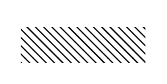
\begin{tikzpicture}
                \path[use as bounding box] (0, 0) rectangle (4em, 1em);
                \fill[pattern=north west lines] (-0.25em, -0.25em) rectangle (4.25em, 1em);
              \end{tikzpicture}
            \\\hline
              \lambda \conjtrsps{\vecv_{1}} \vecu & \multirow{3}{*}{
                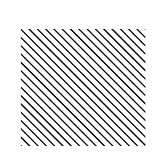
\begin{tikzpicture}
                  \path[use as bounding box] (0, 0) rectangle (4em, 4em);
                  \fill[pattern=north west lines] (-0.25em, -0.25em) rectangle (4.25em, 3.95em);
                \end{tikzpicture}
              }
            \\
              \vdots &
            \\
              \lambda \conjtrsps{\vecv_{n - 1}} \vecu
            \end{genmat}
        \\&=
            \begin{genmat}{c|@{}c@{}}
              \lambda &
              
\begin{tikzpicture}
                \path[use as bounding box] (0, 0) rectangle (4em, 1em);
                \fill[pattern=north west lines] (0.1em, -0.25em) rectangle (4em, 1em);
              \end{tikzpicture}
            \\\hline
              \expandV{\veczero} & \expandHV{A'}
            \end{genmat}
        \end{align*}
        を満たす.ここで $A' \in \setMatrix{\paren{n - 1}}{\paren{n - 1}}{\setC}$ とおいた行列に対し,
        帰納法の仮定より或るユニタリ行列 $Q' \in \setMatrix{\paren{n - 1}}{\paren{n - 1}}{\setC}$ と
        上三角行列 $R' \in \setMatrix{\paren{n - 1}}{\paren{n - 1}}{\setC}$ が存在して $\conjtrsps{Q'} A' Q' = R'$ が成り立つ.
        この $Q'$ を用いて
        $\DS Q \defeq
          \begin{genmat}{c|c}
            1 & \trsps{\veczero}
          \\\hline
            \veczero & \expandHV{Q'}
          \end{genmat}
        $
        とすると $Q$ は明らかにユニタリ行列で
        \begin{align*}
          \conjtrsps{Q} A Q
          =
            \begin{genmat}{c|c}
              1 & \trsps{\veczero}
            \\\hline
              \veczero & \expandHV{\conjtrsps{Q'}}
            \end{genmat}
            \begin{genmat}{c|@{}c@{}}
              \lambda &
              
\begin{tikzpicture}
                \path[use as bounding box] (0, 0) rectangle (4em, 1em);
                \fill[pattern=north west lines] (0.1em, -0.25em) rectangle (4em, 1em);
              \end{tikzpicture}
            \\\hline
              \expandV{\veczero} & \expandHV{A'}
            \end{genmat}
            \begin{genmat}{c|c}
              1 & \trsps{\veczero}
            \\\hline
              \veczero & \expandHV{Q'}
            \end{genmat}
          &=
          \begin{genmat}{c|@{}c@{}}
            \lambda &
              
\begin{tikzpicture}
                \path[use as bounding box] (0, 0) rectangle (4em, 1em);
                \fill[pattern=north west lines] (0.1em, -0.25em) rectangle (4em, 1em);
              \end{tikzpicture}
          \\\hline
            \veczero & \expandHV{R'}
          \end{genmat}
          \backdefeq R
        \end{align*}
        となり,これは上三角行列である.
      \end{itemize}
      以上より,$\conjtrsps{Q} A Q = R$ なるユニタリ行列 $Q$ と上三角行列 $R$ が存在する.\qed
    }
    \defpar{Schur標準形}{
      複素正方行列 $A$ に対して定理~\ref{thm:trans-by-unitary-into-uptriangle}により存在する $R$ は,
      $A$ の\newword{Schur標準形}と呼ばれる.
    }
    \lempar{}{
      複素正方行列 $A$ のSchur標準形 $R$ の対角成分は $A$ の固有値である.
    }
    \proof{}{
      定理~\ref{thm:trans-by-unitary-into-uptriangle}より $\conjtrsps{Q} A Q = R$ なるユニタリ行列 $Q$ が存在する.
      この $Q$ を用いると
      \begin{align*}
        \det \paren{\lambda I - A}
        &= \det \paren{\lambda I - A} \cdot \det I
      \\&= \det \paren{\lambda I - A} \cdot \det \paren{\conjtrsps{Q} Q}
      \\&= \det \paren{\lambda I - A} \cdot \det \conjtrsps{Q} \cdot \det Q
          \holdby{定理~\ref{thm:det-mult-homomorphism}}
      \\&= \det \conjtrsps{Q} \cdot \det \paren{\lambda I - A} \cdot \det Q
      \\&= \det \paren{\conjtrsps{Q} \paren{\lambda I - A} Q}
          \holdby{定理~\ref{thm:det-mult-homomorphism}}
      \\&= \det \paren{\lambda I - \conjtrsps{Q} A Q}
      \\&= \det \paren{\lambda I - R}
      \\&= \prod_{i = 1}^{n} \paren{\lambda - R_{i i}}
          \holdby{$R$ は上三角行列}
      \end{align*}
      であるから,確かに $R$ の各対角成分は重複度も含めて $A$ の固有値に一致する.\qed
    }
    \thmpar{}{
      正規行列 $A \in \setMatrix{n}{n}{K}$ に対し,
      或るユニタリ行列 $Q \in \setMatrix{n}{n}{K}$ と対角行列 $\Lambda \in \setMatrix{n}{n}{K}$ が存在して
      $\conjtrsps{Q} A Q = \Lambda$ が成り立つ.
    }
    \proof{}{
      \subproof{$\limpl$}{
        定理~\ref{thm:trans-by-unitary-into-uptriangle}より或るユニタリ行列 $Q$ と上三角行列 $R$ が存在して
        $\conjtrsps{Q} A Q = R$ が成り立つ.この $R$ が対角行列であることを示せばよい.
        \begin{align*}
          R \conjtrsps{R}
          = \paren{\conjtrsps{Q} A Q} \paren{\conjtrsps{Q} \conjtrsps{A} Q}
          = \conjtrsps{Q} A \paren{Q \conjtrsps{Q}} \conjtrsps{A} Q
          &= \conjtrsps{Q} A \conjtrsps{A} Q
            \holdby{$Q$ はユニタリ行列}
        \\&= \conjtrsps{Q} \conjtrsps{A} A Q
            \holdby{$A$ は正規行列}
        \\&= \conjtrsps{Q} \conjtrsps{A} \paren{Q \conjtrsps{Q}} A Q
            \holdby{$Q$ はユニタリ行列}
        \\&= \paren{Q \conjtrsps{A} Q} \paren{\conjtrsps{Q} A Q}
          = \conjtrsps{R} R
        \end{align*}
        より $R$ も正規行列である.ここで
        $\DS R =
          \begin{genmat}{@{}ccc@{}}
            \lambda_{1} & &
              
\begin{tikzpicture}
                \path[use as bounding box] (0, 0) rectangle (-1em, -1em);
                \fill[pattern=north west lines] (0, 0) -- (-4.8em, 0) -- (0, -4.1em) -- cycle;
              \end{tikzpicture}
          \\
            & \ddots &
          \\
            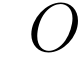
\begin{tikzpicture}
              \path[use as bounding box] (0, 0) rectangle (1em, 1em);
              \draw node at (1em, 1em) {\Huge $O$};
            \end{tikzpicture}
            & & \lambda_{n}
          \end{genmat}
        $
        とおくと,$R \conjtrsps{R} = \conjtrsps{R} R$ より
        \begin{align*}
            \begin{genmat}{@{}ccc@{}}
              \lambda_{1} & &
                
\begin{tikzpicture}
                  \path[use as bounding box] (0, 0) rectangle (-1em, -1em);
                  \fill[pattern=north west lines] (0, 0) -- (-4.8em, 0) -- (0, -3.9em) -- cycle;
                \end{tikzpicture}
            \\
              & \ddots &
            \\
              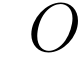
\begin{tikzpicture}
                \path[use as bounding box] (0, 0) rectangle (1em, 1em);
                \draw node at (1em, 1em) {\Huge $O$};
              \end{tikzpicture}
              & & \lambda_{n}
            \end{genmat}
            \begin{genmat}{@{}ccc@{}}
              \conj{\lambda_{1}} & &
                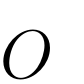
\begin{tikzpicture}
                  \path[use as bounding box] (0, 0) rectangle (-1em, -1em);
                  \draw node at (-1em, -1em) {\Huge $O$};
                \end{tikzpicture}
            \\
              & \ddots &
            \\
              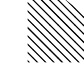
\begin{tikzpicture}
                \path[use as bounding box] (0, 0) rectangle (1em, 1em);
                \fill[pattern=north west lines] (0, -0.25em) -- (4.2em, -0.25em) -- (0, 3.1em) -- cycle;
              \end{tikzpicture}
              & & \conj{\lambda_{n}}
            \end{genmat}
          &=
            \begin{genmat}{@{}ccc@{}}
              \conj{\lambda_{1}} & &
                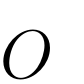
\begin{tikzpicture}
                  \path[use as bounding box] (0, 0) rectangle (-1em, -1em);
                  \draw node at (-1em, -1em) {\Huge $O$};
                \end{tikzpicture}
            \\
              & \ddots &
            \\
              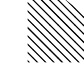
\begin{tikzpicture}
                \path[use as bounding box] (0, 0) rectangle (1em, 1em);
                \fill[pattern=north west lines] (0, -0.25em) -- (4.2em, -0.25em) -- (0, 3.1em) -- cycle;
              \end{tikzpicture}
              & & \conj{\lambda_{n}}
            \end{genmat}
            \begin{genmat}{@{}ccc@{}}
              \lambda_{1} & &
                
\begin{tikzpicture}
                  \path[use as bounding box] (0, 0) rectangle (-1em, -1em);
                  \fill[pattern=north west lines] (0, 0) -- (-4.8em, 0) -- (0, -3.9em) -- cycle;
                \end{tikzpicture}
            \\
              & \ddots &
            \\
              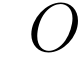
\begin{tikzpicture}
                \path[use as bounding box] (0, 0) rectangle (1em, 1em);
                \draw node at (1em, 1em) {\Huge $O$};
              \end{tikzpicture}
              & & \lambda_{n}
            \end{genmat}
        \end{align*}
        であり,%さらに $\rowvec{R}{1} = \begin{genmat}{@{}c|c|c|c@{}} \lambda_{1} & R_{1 2} & \cdot & R_{1 n}\end{genmat}$ より
        両辺の $\seqprn{1, 1}$ 成分の比較により $\rowvec{R}{1} \conjtrsps{\paren{\rowvec{R}{1}}} = \conj{\lambda_{1}} \lambda_{1}$,
        すなわち $\absprn{\lambda_{1}}^{2} + \absprn{R_{1 2}}^{2} + \cdots + \absprn{R_{1 n}}^{2} = \absprn{\lambda_{1}}^{2}$,
        よって $R_{1 2} = \cdots = R_{1 n} = 0$ が成り立つ.第 $2$ 行以降も同様にして非対角成分が $0$ とわかり,
        ゆえに $R$ は対角行列である.\qed
      }
      \subproof{$\backlimpl$}{
        対角行列 $\Lambda$ に対して明らかに $\conjtrsps{\Lambda} \Lambda = \Lambda \conjtrsps{\Lambda}$ が成り立つ.ゆえに
        \begin{align*}
          A \conjtrsps{A}
          = \paren{\conjtrsps{Q} \Lambda Q} \paren{\conjtrsps{Q} \conjtrsps{\Lambda} Q}
          &= \conjtrsps{Q} \Lambda \conjtrsps{\Lambda} Q
            \holdby{$Q$ はユニタリ行列}
        \\&= \conjtrsps{Q} \conjtrsps{\Lambda} \Lambda Q
            \holdby{$\conjtrsps{\Lambda} \Lambda = \Lambda \conjtrsps{\Lambda}$}
        \\&= \paren{\conjtrsps{Q} \conjtrsps{\Lambda} Q} \paren{\conjtrsps{Q} \Lambda Q}
            \holdby{$Q$ はユニタリ行列}
        \\&= \conjtrsps{A} A
        \end{align*}
        であり $A$ は正規行列である.\qed
      }
    }
    \lempar{}{
      Hermite行列の固有値はすべて実数である.
    }
    \proof{}{
      複素正方行列 $A \in \setMatrix{n}{n}{\setC}$ をHermite行列とする.
      $\lambda \in \setC$ が $A$ の固有値,$\vecx \in \setC^{n} \setmns \setprn{\veczero}$ が
      $\lambda$ に対応する固有ベクトルのひとつであるとすると
      \begin{align}
        \conjtrsps{\vecx} A \vecx
        = \conjtrsps{\vecx} \paren{\lambda \vecx}
        = \lambda \conjtrsps{\vecx} \vecx
          \label{eq:eigenval-of-hermite}
      \end{align}
      が成り立つ.ここで\eqref{eq:eigenval-of-hermite}の左辺の複素共軛をとると
      \begin{align*}
        \conj{\conjtrsps{\vecx} A \vecx}
        &= \conjtrsps{\paren{\conjtrsps{\vecx} A \vecx}}
        = \conjtrsps{\vecx} \conjtrsps{A} \vecx
        = \conjtrsps{\vecx} A \vecx
          \holdby{$A$ はHermite行列}
      \end{align*}
      であり,一方で\eqref{eq:eigenval-of-hermite}の右辺も複素共軛をとると
      \begin{align*}
        \conj{\lambda \conjtrsps{\vecx} \vecx}
        &= \conj{\lambda} \conjtrsps{\paren{\conjtrsps{\vecx} \vecx}}
        = \conj{\lambda} \conjtrsps{\vecx} \vecx
      \end{align*}
      であるから $\conjtrsps{\vecx} A \vecx = \conj{\lambda} \conjtrsps{\vecx} \vecx$,
      よって\eqref{eq:eigenval-of-hermite}と合わせて
      $\lambda \conjtrsps{\vecx} \vecx = \conj{\lambda} \conjtrsps{\vecx} \vecx$ が成り立つ.
      $\vecx \neq \veczero$ より $\conjtrsps{\vecx} \vecx \neq 0$ であるから $\lambda = \conj{\lambda}$.
      ゆえに $A$ の固有値は実数である.\qed
    }
  \subsection{固有値計算}
    \defpar{Rayleigh商}{
      Hermite行列 $A \in \setMatrix{n}{n}{\setC}$ に対して
      写像 $\funcdoms{\Rayleigh{A}}{\setC^{n} \setmns \setprn{\veczero}}{\setC}$ を
      \begin{align*}
        \app{\Rayleigh{A}}{\vecx} \defeq \frac{\conjtrsps{\vecx} A \vecx}{\conjtrsps{\vecx} \vecx}
      \end{align*}
      で定める.$\app{\Rayleigh{A}}{x}$ を $A$ による $\vecx$ の\newword{Rayleigh商}と呼ぶ.
    }
    \plainpar{}{
      $A$ の固有値 $\lambda$ と対応する固有ベクトルのひとつ $\vecu$ に対して
      $\app{\Rayleigh{A}}{\vecu} = \lambda$ が成り立つ.
    }
    \thmpar{Courant--Fischerの定理}{
      Hermite行列 $A \in \setMatrix{n}{n}{\setC}$ の固有値 $\lambda_{1} \geq \cdots \geq \lambda_{n}$ に対して
      \begin{align*}
        \lambda_{k} &= \max \setprnsep{\min \setprnsep{\app{\Rayleigh{A}}{\vecx}}{\vecx \in U \setmns \setprn{\veczero}}}{%
          U \in \subspaceof{k}{\setC^{n}, +, \cdot}}
      \\
        \lambda_{k} &= \min \setprnsep{\max \setprnsep{\app{\Rayleigh{A}}{\vecx}}{\vecx \in U \setmns \setprn{\veczero}}}{%
          U \in \subspaceof{k}{\setC^{n}, +, \cdot}}
      \end{align*}
      がそれぞれ成り立つ.
    }
    \proof{}{
      $\lambda_{1}, \ldots, \lambda_{n}$ の各々に対応する規格化された固有ベクトルのひとつをそれぞれ $\vecu_{1}, \ldots, \vecu_{n}$ とおいて
      $V_{k} \defeq \spanop \setprn{\vecu_{1}, \ldots, \vecu_{k}}$,
      $W_{l} \defeq \spanop \setprn{\vecu_{n - l + 1}, \ldots, \vecu_{n}}$
      と定める.このとき,次の副補題が成り立つ:
      \subarea{
        \sublempar{}{
          $\forallin{\vecx}{V_{k} \setmns \setprn{\veczero}}{\lambda_{1} \geq \app{\Rayleigh{A}}{\vecx} \geq \lambda_{k}}$
        }
        \proof{}{
          $\vecx \in V_{k} \setmns \setprn{\veczero}$ とする.
          $\vecx = \alpha_{1} \vecu_{1} + \cdots + \alpha_{k} \vecu_{k}$ とおくと,
          $\vecx \neq \veczero$ より $\conjtrsps{\vecx} \vecx > 0$ であるから
          \begin{align*}
            \app{\Rayleigh{A}}{\vecx}
            = \frac{\conjtrsps{\vecx} A \vecx}{\conjtrsps{\vecx} \vecx}
            &= \frac{\lambda_{1} \absprn{\alpha_{1}}^{2} + \cdots + \lambda_{k} \absprn{\alpha_{k}}^{2}}{%
                \absprn{\alpha_{1}}^{2} + \cdots + \absprn{\alpha_{k}}^{2}}
          \\&\leq \frac{\lambda_{1} \absprn{\alpha_{1}}^{2} + \cdots + \lambda_{1} \absprn{\alpha_{k}}^{2}}{%
                \absprn{\alpha_{1}}^{2} + \cdots + \absprn{\alpha_{k}}^{2}} = \lambda_{1}
              \holdby{$\lambda_{1} \geq \cdots \geq \lambda_{k}$}
          \end{align*}
          であり,$\app{\Rayleigh{A}}{\vecx} \leq \lambda_{1}$ が成り立つ.
          同様にして $\app{\Rayleigh{A}}{\vecx} \geq \lambda_{k}$ も示せる.\qed
        }
        \sublempar{}{
          $\forallin{\vecx}{W_{l} \setmns \setprn{\veczero}}{\lambda_{n - l + 1} \geq \app{\Rayleigh{A}}{\vecx} \geq \lambda_{n}}$
        }
        \proof{}{上と同様.\qed}
      }
      $U \in \subspaceof{k}{\setC^{n}, +, \cdot}$ を任意の $k$ 次元部分空間とすると,まず
      \begin{align*}
        n + 1
        = k + \paren{n - k + 1}
        &= \dim U + \dim W_{n - k + 1}
      \\&= \dim \paren{U + W_{n - k + 1}} + \dim \paren{U \cap W_{n - k + 1}}
      \\&\leq n + \dim \paren{U \cap W_{n - k + 1}}
      \end{align*}
      より $\dim \paren{U \cap W_{n - k + 1}} \geq 1$ であり,
      $\paren{U \cap W_{n - k + 1}} \setmns \setprn{\veczero} \neq \varnothing$ が成り立つ.
      したがって明らかに
      \begin{align*}
        \min \setprnsep{\app{\Rayleigh{A}}{\vecx}}{\vecx \in U \setmns \setprn{\veczero}}
        &\leq \min \setprnsep{\app{\Rayleigh{A}}{\vecx}}{\vecx \in \paren{U \cap W_{n - k + 1}} \setmns \setprn{\veczero}}
      \end{align*}
      であり,また各 $\vecx \in \paren{U \cap W_{n - k + 1}} \setmns \setprn{\veczero}$ に対して
      $\vecx \in W_{n - k + 1}$ と副補題より $\lambda_{k} \geq \app{\Rayleigh{A}}{\vecx}$ が成り立つから
      $\min \setprnsep{\app{\Rayleigh{A}}{\vecx}}{\vecx \in U \setmns \setprn{\veczero}} \leq \lambda_{k}$.
      特に $U \defeq V_{k}$ を代入すれば副補題より等号が成立し,ゆえに
      \begin{align*}
        \max \setprnsep{\min \setprnsep{\app{\Rayleigh{A}}{\vecx}}{\vecx \in U \setmns \setprn{\veczero}}}{
          U \in \subspaceof{k}{\setC^{n}, +, \cdot}}
        &= \lambda_{k}
      \end{align*}
      が成り立つ.\qed
    }
    \corpar{最大固有値と最小固有値のRayleigh商による表現}{
      Hermite行列 $A \in \setMatrix{n}{n}{\setC}$
      の最大固有値を $\lambda_{\mathrm{max}}$,最小固有値を $\lambda_{\mathrm{min}}$ とおくと,
      \begin{align*}
        \lambda_{\mathrm{max}} &= \max \setprnsep{\app{\Rayleigh{A}}{\vecx}}{\vecx \in \setC^{n} \setmns \setprn{\veczero}}
      \\
        \lambda_{\mathrm{min}} &= \min \setprnsep{\app{\Rayleigh{A}}{\vecx}}{\vecx \in \setC^{n} \setmns \setprn{\veczero}}
      \end{align*}
      が成り立つ.
    }
\section{行列の標準形}
  \subsection{標準形のまとめ}
    \plainpar{}{
      ここまでには掲載していないものも含め,本文書で挙げる標準形の一覧を表~\ref{table:standard-form}に掲げる.
      \begin{table}[tbp]
      \centering
        \begin{tabular}{cccc}
        \hlinevar{2pt}
          線型写像の型 & 許容する変換 & 標準形 & 応用例
        \\\hlinevar{1pt}
          $\doms{V}{V}$ & \begin{tabular}{c}\newword{相似変換}:\\正則行列 $S$ を用いて\\$A \mapsto S^{-1} A S$\end{tabular}
            & \begin{tabular}{c}\newword{Frobenius標準形}\\\newword{Jordan標準形}\end{tabular} & 常微分方程式
        \\\hline
          $\doms{V}{V}$ & \begin{tabular}{c}\newword{ユニタリ相似変換}:\\ユニタリ行列 $Q$ を用いて\\$A \mapsto Q^{-1} A Q$\end{tabular}
            & \begin{tabular}{c}\newword{Schur標準形}\\(特に正規行列対角化)\end{tabular} &
        \\\hline
          $\doms{V}{V^{*}}$ & \begin{tabular}{c}\newword{合同変換}:\\正則行列 $S$ を用いて\\$A \mapsto \conjtrsps{S} A S$\end{tabular}
            & \newword{Sylvester標準形} & $2$ 次形式
        \\\hline
          $\doms{V}{U}$ & \begin{tabular}{c}\newword{同値変換}:\\正則行列 $S$,$T$ を用いて\\$A \mapsto S A T$\end{tabular}
            & \newword{階数標準形} & 線型方程式
        \\\hline
          $\doms{V}{U}$ & \begin{tabular}{c}ユニタリ同値変換:\\ユニタリ行列 $P$,$Q$ を用いて\\$A \mapsto P A Q$\end{tabular}
            & \newword{特異値標準形} &
        \\\hlinevar{2pt}
        \end{tabular}
        \caption{標準形のまとめ}\label{table:standard-form}
      \end{table}
    }
    \defpar{Sylvester標準形}{
      Hermite行列 $A \in \setMatrix{n}{n}{\setC}$ に対して
      正則行列 $S \in \setMatrix{n}{n}{\setC}$ を用いて変形される
      \begin{align*}
        A' = \conjtrsps{S} A S
        &=
        \begin{genmat}{@{}c@{}|c}
          \begin{array}{c|c}
            I_{s} & O
          \\\hline
            O & -I_{t}
          \end{array}
          & O
        \\\hline
          O & O
        \end{genmat}
      \end{align*}
      の形を $A$ の\newword{Sylvester標準形}と呼ぶ.なお,この $s$ と $t$ は $s + t = \rank A$ を満たす.
    }
    \defpar{特異値標準形}{
      行列 $A \in \setMatrix{m}{n}{\setC}$ に対し,ユニタリ行列 $P \in \setMatrix{m}{m}{\setC}$ と $Q \in \setMatrix{n}{n}{\setC}$ を
      用いて変形される
      \begin{align*}
        A' = P A Q
        &=
          \begin{genmat}{@{}c@{}|c}
            \begin{array}{ccc}
              \sigma_{1} & &
                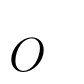
\begin{tikzpicture}
                  \path[use as bounding box] (0, 0) rectangle (1em, 1em);
                  \draw (0, 0) node {\LARGE $O$};
                \end{tikzpicture}
            \\
              & \ddots &
            \\
                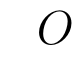
\begin{tikzpicture}
                  \path[use as bounding box] (0, 0) rectangle (-1em, -1em);
                  \draw (0, 0) node {\LARGE $O$};
                \end{tikzpicture}
              & & \sigma_{r}
            \end{array}
            & O
          \\\hline
            O & O
          \end{genmat}
      \end{align*}
      の形を $A$ の特異値標準形と呼ぶ.$\sigma_{1}, \ldots, \sigma_{r}$ を $A$ の\newword{特異値}と呼び,
      これらは $\sigma_{1} \geq \cdots \geq \sigma_{r}$ となるように $P$ と $Q$ を選んで並べ替えられる.
    }
    \lempar{}{
      $A \in \setMatrix{m}{n}{\setC}$ の $\sigma_{1} \geq \cdots \geq \sigma_{r}$ なる特異値 $\sigma_{1}, \ldots, \sigma_{r}$ に対して
      \begin{align*}
        \sigma_{k} &=
          \max \setprnsep{\min \setprnsep{\frac{\norm{A \vecx}}{\norm{\vecx}}}{\vecx \in W \setmns \setprn{\veczero}}}{
            W \in \subspaceof{k}{\setC^{n}, +, \cdot}}
      \end{align*}
      が成り立つ.
    }
    \proof{}{
      $H \defeq \conjtrsps{A} A$ とおくと,任意の $\vecx \in \setcolvec{\setC}{n}$ に対して
      $\conjtrsps{\vecx} H \vecx = \norm{A \vecx}^{2} \geq 0$ であるから $H$ は半正定値.よって対角化
      \begin{align*}
        Q^{-1} H Q &=
          \begin{genmat}{@{}c@{}|c}
            \begin{array}{ccc}
              \lambda_{1} & &
            \\
              & \ddots &
            \\
              & & \lambda_{r}
            \end{array}
            & O
          \\\hline
            O & O
          \end{genmat}
      \end{align*}
      に対して $\forallin{k}{\Natleq{r}}{\lambda_{k} \geq 0}$ が成り立つ.
    }
  \TODO{Jordan標準形}
  \TODO{Frobenius標準形}
  \TODO{多項式行列(重い)}
\section{グラフと行列}
  \subsection{強連結成分分解}
    \defpar{置換行列}{
      各行各列にちょうど $1$ 個 $1$ があって,その他の成分は $0$ であるような正方行列を\newword{置換行列}と呼ぶ.
    }
  \subsection{二部グラフ}
    \plainpar{}{
      証明せず紹介のみに留まる形になるが,二部グラフに関する重要な定理を掲げる.
    }
    \defpar{二部グラフ,マッチング,完全マッチング}{
      $U \cap V = \varnothing$ なる有限集合 $U$,$V$ と
      二項関係 $E \subseteq U \times V$ の組 $G = \seqprn{U, V; E}$ を\newword{二部グラフ}と呼ぶ.
      二部グラフ $G= \seqprn{U, V; E}$ と $X \subseteq U$ に対して
      \begin{align*}
        \app{\Gamma}{X} \defeq \setprnsep{v \in V}{\existsin{x}{X}{\seqprn{x, v} \in E}}
      \end{align*}
      で $\app{\Gamma}{X}$ を定める.$F \subseteq E$ に対して
      \begin{align*}
        \partial F \defeq \setprnsep{u \in U}{\existsin{v}{V}{\seqprn{u, v} \in E}} \cup \setprnsep{v \in V}{\existsin{u}{U}{\seqprn{u, v} \in E}}
      \end{align*}
      で $\partial F$ を定義する.$K \subseteq U$ と $L \subseteq V$ が
      $\forallin{\seqprn{u, v}}{E}{\lflor{u \in K}{v \in L}}$ を満たすとき,$\seqprn{K, L}$ を $G$ の\newword{被覆}と呼ぶ.
      また,二部グラフ $G = \seqprn{U, V; E}$ に対し,$M \subseteq E$ が $\card{\partial M} = 2 \card{M}$ を満たすとき,
      $M$ を $G$ 上の\newword{マッチング}と呼び,特に $\card{U} = \card{V}$ なる二部グラフ $G = \seqprn{U, V; E}$ に対して
      $G$ 上のマッチング $M$ が $\card{M} = \card{U} = \card{V}$ を満たすとき,$M$ を $G$ 上の\newword{完全マッチング}と呼ぶ.
    }
    \thmpar[thm:koenig]{K\"onigの定理}{
      二部グラフ $G = \seqprn{U, V; E}$ に対して
      \begin{align*}
        \max \setprnsep{\card{M}}{\text{$M$ は $G$ のマッチング}}
        =
        \min \setprnsep{\card{K} + \card{L}}{\text{$\seqprn{K, L}$ は $G$ の被覆}}
      \end{align*}
      が成り立つ.
    }
    \proof{}{
      省略する.
    }
    \thmpar[thm:hall]{Hallの定理}{
      $\card{U} = \card{V}$ なる二部グラフ $G = \seqprn{U, V; E}$ に対し,$G$ に完全マッチングが存在することと
      \begin{align*}
        \forallsub[1]{X}{U}{\card{\app{\Gamma}{X}} \geq \card{X}}
      \end{align*}
      が成り立つことは同値.
    }
    \proof{}{省略する.}
    \thmpar[thm:hall-ore]{Hall--Oreの定理}{
      二部グラフ $G = \seqprn{U, V; E}$ に対して
      \begin{align*}
        \max \setprnsep{\card{M}}{\text{$M$ は $G$ のマッチング}}
        =
        \min \setprnsep{\card{\app{\Gamma}{X}} - \card{X}}{X \subseteq U} + \card{U}
      \end{align*}
      が成り立つ.
    }
    \proof{}{省略する.}
  \subsection{Dulmage--Mendelsohn分解}
    \lempar{}{
      二部グラフ $G = \seqprn{U, V; E}$ に対して $\app{f_{G}}{X} \defeq \card{\app{\Gamma}{X}} - \card{X}$ で
      $\funcdoms{f_{G}}{\Power{U}}{\setZ}$ を定めると,$f_{G}$ は\newword{劣模律}:
      \begin{align*}
        \forallsub[1]{X|Y}{U}{\app{f_{G}}{X} + \app{f_{G}}{Y} \geq \app{f_{G}}{X \cap Y} + \app{f_{G}}{X \cup Y}}
      \end{align*}
      を満たす.
    }
    \lempar{最小化集合族の $\cap$, $\cup$-閉性}{
      二部グラフ $G = \seqprn{U, V; E}$ に対して $f_{G}$ を最小化する集合全体からなる集合族を $\Dminzr{f_{G}}$,すなわち
      $\Dminzr{f_{G}} \defeq \setprnsep{X \subseteq U}{\forallsub{Y}{U}{\app{f_{G}}{X} \leq \app{f_{G}}{Y}}}$
      とおくと,
      \begin{align*}
        \forallin{X|Y}{\Dminzr{f_{G}}}{\lfland{X \cap Y \in \Dminzr{f_{G}}}{X \cup Y \in \Dminzr{f_{G}}}}
      \end{align*}
      が成り立つ.
    }
    \proof{}{
      $f_{G}$ の最小値を $\alpha$,すなわち $\alpha \defeq \min \setprnsep{\app{f_{G}}{Z}}{Z \subseteq U}$ とおき,
      $X, Y \in \Dminzr{f_{G}}$ とする.
      仮に $X \cap Y \not\in \Dminzr{f_{G}}$ であるとすると,$\app{f_{G}}{X \cap Y} > \alpha$ であるが,
      劣模律より
      \begin{align*}
        2 \alpha = \app{f_{G}}{X} + \app{F_{G}}{Y} \geq \app{f_{G}}{X \cap Y} + \app{f_{G}}{X \cup Y}
      \end{align*}
      であるから $\app{f_{G}}{X \cup Y} \leq 2 \alpha - \app{f_{G}}{X \cap Y} < \alpha$ となり,$\alpha$ の定義に矛盾.
      ゆえに $X \cap Y \in \Dminzr{f_{G}}$.劣模律の対称性より $X \cup Y$ についても同様である.\qed
    }
    \defpar{Dulmage--Mendelsohn分解}{
      二部グラフ $G = \seqprn{U, V; E}$ に対し,$\seqprn{\Dminzr{f_{G}}, \cap, \cup}$ の極大鎖のひとつ,
      $X_{0} \subsetcovered X_{1} \subsetcovered \cdots \subsetcovered X_{b}$ なる $\seqprn{X_{k}}_{k = 0}^{b}$ を用いて
      \begin{align*}
        U_{k} &\defeq
          \begin{cases}
            X_{0}                   &\caseif{k = 0}
          \\
            X_{k} \setmns X_{k - 1} &\caseif{k \in \Natleq{b}}
          \\
            U \setmns X_{b}         &\caseif{k = \infty}
          \end{cases}
      &
        V_{k} &\defeq
          \begin{cases}
            \app{\Gamma}{X_{0}}                                 &\caseif{k = 0}
          \\
            \app{\Gamma}{X_{k}} \setmns \app{\Gamma}{X_{k - 1}} &\caseif{k \in \Natleq{b}}
          \\
            V \setmns \app{\Gamma}{X_{b}}                       &\caseif{k = \infty}
          \end{cases}
      \end{align*}
      で $\seqprn{U_{k}}_{\scriptrange{k \in \setprn{0} \cup \Natleq{b} \cup \setprn{\infty}}}$
      と $\seqprn{V_{k}}_{\scriptrange{k \in \setprn{0} \cup \Natleq{b} \cup \setprn{\infty}}}$ を定める.
      これらの集合列の組を $G$ の\newword{Dulmage--Mendelsohn分解}と呼ぶ.
    }
    \begin{figure}[tb]
    \centering
      {\def\drawline#1#2{\draw[line width=1pt] (0, #1) -- (6, #2)}%
       \def\drawUellipse#1#2#3#4{\draw ($(0, #1)!0.5!(0, #2)$) ellipse[y radius=#3,x radius=#4]}%
       \def\drawVellipse#1#2#3#4{\draw ($(6, #1)!0.5!(6, #2)$) ellipse[y radius=#3,x radius=#4]}%
       \def\drawUnode#1#2#3{\draw (-1.1, #1) -- (-1.25, #1) -- (-1.25, #2) node[midway,left=0.25em] {#3} -- (-1.1, #2)}%
       \def\drawVnode#1#2#3{\draw (7.1, #1) -- (7.25, #1) -- (7.25, #2) node[midway,right=0.25em] {#3} -- (7.1, #2)}%
      \begin{tikzpicture}
        \drawline{0}{0};
        \drawline{1}{0};
        \drawline{2}{0};
        \drawline{2}{1};
        \drawline{3}{0};
        \drawline{3}{1};
        \drawline{3}{2};
        \drawline{4}{1};
        \drawline{4}{3};
        \drawline{4}{4};
        \drawline{5}{3};
        \drawline{5}{4};
        \drawline{6}{2};
        \drawline{6}{5};
        \drawline{6}{6};
        \drawUellipse{0}{1}{0.75}{0.2};
        \drawUellipse{0}{2}{1.35}{0.4};
        \drawUellipse{0}{3}{1.95}{0.6};
        \drawUellipse{0}{5}{3.05}{0.85};
        \drawVellipse{0}{0}{0.2}{0.2};
        \drawVellipse{0}{1}{0.8}{0.4};
        \drawVellipse{0}{2}{1.4}{0.6};
        \drawVellipse{0}{4}{2.5}{0.85};
        \foreach \Ypos in {0,1,2,3,4,5,6} \fill[color=black] (0, \Ypos) circle[radius=2pt];
        \foreach \Ypos in {0,1,2,3,4,5,6} \fill[color=black] (6, \Ypos) circle[radius=2pt];
        \draw (0, 7) node {$U$};
        \draw (6, 7) node {$V$};
        \drawUnode{-0.3}{1.3}{$U_{0}$};
        \drawUnode{1.7}{2.3}{$U_{1}$};
        \drawUnode{2.7}{3.3}{$U_{2}$};
        \drawUnode{3.7}{5.3}{$U_{3}$};
        \drawUnode{5.7}{6.3}{$U_{\infty}$};
        \drawVnode{-0.3}{0.3}{$V_{0}$};
        \drawVnode{0.7}{1.3}{$V_{1}$};
        \drawVnode{1.7}{2.3}{$V_{2}$};
        \drawVnode{2.7}{4.3}{$V_{3}$};
        \drawVnode{4.7}{6.3}{$V_{\infty}$};
      \end{tikzpicture}}
      \caption{Dulmage--Mendelsohn分解の例}\label{fig:dm-decomp}
    \end{figure}
    \plainpar{}{
      Dulmage--Mendelsohn分解の例を図~\ref{fig:dm-decomp}に掲げる.
      また,以下に掲げる補題は $\Dminzr{f_{G}}$ の性質より直観的にも簡単に導かれる.
    }
    \lempar{}{
      二部グラフ $G = \seqprn{U, V; E}$ のDulmage--Mendelsohn分解
      $\seqprn{\seqprn{U_{k}}_{\scriptrange{k \in \setprn{0} \cup \Natleq{b} \cup \setprn{\infty}}},
               \seqprn{V_{k}}_{\scriptrange{k \in \setprn{0} \cup \Natleq{b} \cup \setprn{\infty}}}}$
      に対し,以下がそれぞれ成り立つ:
      \begin{thmenum}
      \thmenumitem\label{lem:dm-decomp-fundamental|1}
        $\forallin{k}{\Natleq{b}}{\card{U_{k}} = \card{V_{k}}}$
      \thmenumitem\label{lem:dm-decomp-fundamental|2}
        $\lflor{\card{U_{0}} > \card{V_{0}}}{\card{U_{0}} = \card{V_{0}} = 0}$
      \end{thmenum}
    }
    \proof{}{
      \subproof{\ref{lem:dm-decomp-fundamental|1}}{
        $\seqprn{\seqprn{U_{k}}_{\scriptrange{k \in \setprn{0} \cup \Natleq{b} \cup \setprn{\infty}}},
         \seqprn{V_{k}}_{\scriptrange{k \in \setprn{0} \cup \Natleq{b} \cup \setprn{\infty}}}}$
        を形成するのに使われた $\seqprn{\Dminzr{f_{G}}, \cap, \cup}$ の極大鎖を $\seqprn{X_{k}}_{k = 0}^{b}$ とおき,
        また $\alpha \defeq \min \setprnsep{\app{f_{G}}{X}}{X \subseteq U}$,すなわち $f_{G}$ の最小値を $\alpha$ とおく.
        このとき $k \in \Natleq{b}$ に対して
        \begin{align*}
          \card{V_{k}}
          = \card{\app{\Gamma}{X_{k}} \setmns \app{\Gamma}{X_{k - 1}}}
          &= \card{\app{\Gamma}{X_{k}}} - \card{\app{\Gamma}{X_{k - 1}}}
            \holdby{$X_{k - 1} \subseteq X_{k}$ より $\app{\Gamma}{X_{k - 1}} \subseteq \app{\Gamma}{X_{k}}$}
        \\&= \paren{\app{f_{G}}{X_{k}} + \card{X_{k}}} - \paren{\app{f_{G}}{X_{k - 1}} + \card{X_{k - 1}}}
        \\&= \paren{\alpha + \card{X_{k}}} - \paren{\alpha + \card{X_{k - 1}}}
            \holdby{$X_{k}, X_{k - 1} \in \Dminzr{f_{G}}$}
        \\&= \card{X_{k}} - \card{X_{k - 1}}
          = \card{X_{k} \setmns X_{k - 1}}
            \holdby{$X_{k - 1} \subseteq X_{k}$}
        \\&= \card{U_{k}}
        \end{align*}
        であり,$\card{U_{k}} = \card{V_{k}}$.\qed
      }
      \subproof{\ref{lem:dm-decomp-fundamental|2}}{
        $\app{f_{G}}{\varnothing} = \card{\app{\Gamma}{\varnothing}} - \card{\varnothing} = 0$ と $\alpha$ の定義より $\alpha \leq 0$ である.
        したがって
        \begin{align*}
          \card{V_{0}} - \card{U_{0}}
          = \card{\app{\Gamma}{X_{0}}} - \card{X_{0}}
          = \app{f_{G}}{X_{0}}
          &= \alpha
            \holdby{$X_{0} \in \Dminzr{f_{G}}$}
        \\&\leq 0
        \end{align*}
        であり,$\card{U_{0}} < \card{V_{0}}$ または $\card{U_{0}} = \card{V_{0}}$ が成り立つ.
        $\card{U_{0}} = \card{V_{0}}$ が成り立つとき,
        $\alpha = \card{V_{0}} - \card{U_{0}} = 0$ であるから $\app{f_{G}}{\varnothing} = 0 = \alpha$,
        すなわち $\varnothing \in \Dminzr{f_{G}}$ が成り立つ.このとき $\seqprn{\Dminzr{f_{G}}, \cap, \cup}$ の極大鎖は
        最小元 $\varnothing$ を含まなければ極大性に反するから,$X_{0} = \varnothing$ が成り立ち,よって
        $\card{V_{0}} = \card{U_{0}} = \card{X_{0}} = \card{\varnothing} = 0$.
        ゆえに $\card{U_{0}} < \card{V_{0}}$ または $\card{U_{0}} = \card{V_{0}} = 0$ が成り立つ.\qed
      }
    }
    \plainpar{}{
      Dulmage--Mendelsohn分解には,ブロック三角化の手法としての意義がある.行列 $A \in \setMatrix{m}{n}{K}$ に対して
      $U \defeq \Natleq{m}$,$V \defeq \Natleq{n}$,$E \defeq \setprnsep{\seqprn{i, j} \in U \times V}{A_{i j} \neq 0}$ で
      二部グラフ $G = \seqprn{U, V; E}$ を定め,これに対してDulmage--Mendelsohn分解
      $\seqprn{\seqprn{U_{k}}_{\scriptrange{k \in \setprn{0} \cup \Natleq{b} \cup \setprn{\infty}}},
               \seqprn{V_{k}}_{\scriptrange{k \in \setprn{0} \cup \Natleq{b} \cup \setprn{\infty}}}}$
      を与えたとする.このとき,もとの行列 $A$ の行と列をこのDulmage--Mendelsohn分解に基づいて並べ替えると,
      $k < l$ なる $k, l \in \setprn{0} \cup \Natleq{b} \cup \setprn{\infty}$ に対して
      $U_{k}$ の元から $V_{l}$ の元へは $G$ 上で辺が存在しないから,
      $A$ を並べ替えた行列の上ではすべての成分が $0$ のブロックに対応する.
      すなわち,図~\ref{fig:block-lower-triangle}のように行列 $A$ のブロック下三角化ができていることになる.
    }
    \begin{figure}[tb]
      {\def\slashes#1#2#3#4#5#6{
         \begin{tikzpicture}
           \path[use as bounding box] (0, 0) rectangle (#1, #2);
           \fill[pattern=north west lines] (#3, #5) rectangle (#4, #6);
         \end{tikzpicture}
       }%
       \def\varslashes#1#2#3#4#5#6{
         \begin{tikzpicture}
           \path[use as bounding box] (0, 0) rectangle (#1, #2);
           \fill[pattern=north west lines] (#3, #5) rectangle (#4, #6);
         \end{tikzpicture}
       }%
       \def\enclosedbylines#1{\multicolumn{1}{@{}|@{}c@{}|@{}}{#1}}%
       \def\leftline#1{\multicolumn{1}{@{}|@{}c@{}}{#1}}%
       \def\rightline#1{\multicolumn{1}{@{}c@{}|@{}}{#1}}%
      \begin{align*}
        P A Q =
        \begin{array}{c@{}r@{}c@{}c@{}c@{}c@{}c@{}l}
          & & V_{0} & V_{1} & V_{2} & \cdots & V_{\infty} &
        \\
          U_{0} & \multirow{5}{*}{\smash{\raisebox{-0.25em}{$\DS\left(\rule[-2.7em]{0pt}{6.5em}\right.$}}} &
            \rightline{\varslashes{2em}{1em}{0em}{1.9em}{-0.3em}{0.9em}} & & &
          &
            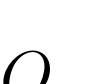
\begin{tikzpicture}
              \path[use as bounding box] (0, 0) -- (2em, 1em);
              \draw (0, -0.75em) node {\Huge $O$};
            \end{tikzpicture}
          & \multirow{5}{*}{\smash{\raisebox{-0.25em}{$\DS\left.\rule[-2.7em]{0pt}{6.5em}\right)$}}}
        \\\cline{3-4}
          U_{1} & &
            \slashes{2em}{1em}{0em}{1.9em}{-0.5em}{0.9em} & \enclosedbylines{\varslashes{2em}{1em}{0.1em}{1.9em}{-0.3em}{0.9em}} & & &
          &
        \\\cline{4-5}
          U_{2} & &
              \slashes{2em}{1em}{0em}{2.1em}{-0.5em}{0.9em}
            & \slashes{2em}{1em}{0em}{1.9em}{-0.5em}{0.9em}
            & \enclosedbylines{\varslashes{2em}{1em}{0.1em}{1.9em}{-0.3em}{0.9em}} & &
          &
        \\\cline{5-5}
          \smash{\text{\raisebox{-0.25em}{$\vdots$}}} & &
              \slashes{2em}{1em}{0em}{2.1em}{-0.5em}{0.9em}
            & \slashes{2em}{1em}{0em}{2.1em}{-0.5em}{0.9em}
            & \slashes{2em}{1em}{0em}{2em}{-0.5em}{0.9em}
            & \smash{\text{\raisebox{-0.25em}{$\ddots$}}} &
          &
        \\\cline{7-7}
          U_{\infty} & &
              \slashes{2em}{1em}{0em}{2.1em}{-0.3em}{0.9em}
            & \slashes{2em}{1em}{0em}{2.1em}{-0.3em}{0.9em}
            & \slashes{2em}{1em}{0em}{2.1em}{-0.3em}{0.9em}
            & \slashes{2em}{1em}{0em}{1.9em}{-0.3em}{0.9em}
            & \leftline{\varslashes{2em}{1em}{0.1em}{2em}{-0.3em}{0.9em}}
          &
        \end{array}
      \end{align*}}
      \caption{Dulmage--Mendelsohn分解による行列のブロック下三角化}\label{fig:block-lower-triangle}
    \end{figure}
\section{非負行列}
  \subsection{既約行列}
    \defpar{既約性}{
      正方行列 $A \in \setMatrix{n}{n}{K}$ に対し,$A$ を零・非零で隣接行列とみた有向グラフが強連結であるとき,
      $A$ は\newword{既約}であるという.
    }
    \lempar[lem:irreducible-to-positive]{}{
      既約な非負正方行列 $A \in\setMatrix{n}{n}{\setR}$ に対し,$\paren{I + A}^{n - 1}$ は正正方行列である.
    }
    \proof{}{
      任意の $\vecx \neq \veczero$ かつ $\vecx \geq \veczero$ なる $\vecx \in \setcolvec{\setR}{n}$ に対して
      $\paren{I + A}^{n - 1} \vecx > \veczero$ を示せばよい.
      \begin{itemize}
      \item $\vecx$ のすべての成分が非零であるとき,すなわち $\vecx > \veczero$ が成り立つとき,
        $\vecy \defeq \paren{I + A} \vecx$ とおくと $\vecy = \vecx + A \vecx$,
        $\vecx > \veczero$,および $A$ の既約性より $A$ はどの行にも正の成分を少なくともひとつもつから $A \vecx > \veczero$.
        ゆえに $\vecy > \veczero$ であり,$\vecy$ もすべての成分が非零である.
      \item $\vecx$ が $0$ を成分にもつとき,積と既約性は対応する行・列の交換で保存するから
        $\DS \vecx =
          \begin{genmat}{@{}c@{}}
            \vecx'
          \\\hline
            \veczero
          \end{genmat}$,
        $\vecx' > \veczero$ として一般性を失わない.やはり $\vecy \defeq \paren{I + A} \vecx$ とおくと
        \begin{align*}
          \vecy
          =
            \begin{genmat}{@{}c@{}}
              \vecy^{(1)}
            \\\hline
              \vecy^{(2)}
            \end{genmat}
          =
            \begin{genmat}{@{}c@{}}
              \vecx'
            \\\hline
              \veczero
            \end{genmat}
            +
            \begin{genmat}{c|c}
              A^{(1 1)} & A^{(1 2)}
            \\\hline
              A^{(2 1)} & A^{(2 2)}
            \end{genmat}
            \begin{genmat}{@{}c@{}}
              \vecx'
            \\\hline
              \veczero
            \end{genmat}
          =
            \begin{genmat}{@{}c@{}}
              \vecx' + A^{(1 1)} \vecx'
            \\\hline
              A^{(2 1)} \vecx'
            \end{genmat}
        \end{align*}
        である.$\vecy^{(1)}$ は上と同様の議論により $\vecy^{(1)} > \veczero$ である.
        ここで $A$ の既約性により $A^{(2 1)}$ には非零成分が存在し,$\vecx' > \veczero$ より
        $A^{(2 1)} \vecx' \neq \veczero$ かつ $A^{(2 1)} \vecx' \geq \veczero$ が成り立つ.
        よって $\vecy^{(2)}$ は非零成分をもち,$\vecy$ の非零成分の個数は $\vecx$ のそれよりも真に多い.
      \end{itemize}
      以上より $I + A$ を左から乗じることでベクトルの非零成分の個数は $n$ 未満の場合真に多くなりちょうど $n$ の場合は $n$ 個のままである.
      “初期値”である $\vecx$ の非零成分は少なくとも $1$ 個あるので,$\paren{I + A}^{n - 1} \vecx$ はすべて非零成分である.
      ゆえに $\vecx \neq \veczero$ かつ $\vecx \geq \veczero$ なるベクトル $\vecx$ に対して
      $\paren{I + A}^{n - 1} \vecx > \veczero$ が成り立ち,$\paren{I + A}^{n - 1}$ は正正方行列である.\qed
    }
    \thmpar[thm:perron-frobenius]{Perron--Frobeniusの定理}{
      既約な非負正方行列は,正ベクトルを固有ベクトルとする正の固有値をもつ.
    }
    \proof{}{
      \begin{align*}
        \app{\mu_{A}}{\vecx}
        &\defeq \max \setprnsep{\lambda \in \setR}{A \vecx - \lambda \vecx \geq \veczero}
      \\&\afterdefeq \min \setprnsep{\frac{\paren{A \vecx}_{i}}{\vecx_{i}}}{\lfland{i \in \Natleq{n}}{\vecx_{i} > 0}}
      \end{align*}
      で $\funcdoms{\mu_{A}}{\setcolvec{\setR}{n} \setmns \setprn{\veczero}}{\setR}$ を定める.また,
      \begin{align*}
        \alpha &\defeq \sup \setprnsep{\app{\mu_{A}}{\vecx}}{
          \lfland{\vecx \in \setcolvec{\setR}{n}}{\lfland{\vecx \geq \veczero}{\vecx \neq \veczero}}}
      \end{align*}
      で $\alpha$ を定めると,$\mu_{A}$ はスカラー倍について保存,すなわち
      $\forallin{\vecx}{\setcolvec{\setR}{n}}{\forallin{k}{\setR \setmns \setprn{0}}{\app{\mu_{A}}{\vecx} = \app{\mu_{A}}{k \vecx}}}$
      を満たすから,$S \defeq \setprnsep{\vecx \in \setcolvec{\setR}{n}}{\lfland{\vecx \neq \veczero}{\norm{\vecx} = 1}}$ とおいて
      $\alpha = \sup \setprnsep{\app{\mu_{A}}{\vecx}}{\vecx \in S}$ と規格化してよい.
      また $\app{\mu_{A}}{\vecone} = \min \setprnsep{\paren{A \vecone}_{i}}{i \in \Natleq{n}}$ は
      $A$ の行和のうち最小のものであるが,$A$ の既約性よりどの行にも非零成分があるので $\app{\mu_{A}}{\vecone} > 0$.
      したがって $\alpha$ の定義より $\alpha \geq \app{\mu_{A}}{\vecone} > 0$ が成り立つ.
      $S$ は $\setcolvec{\setR}{n}$ 上の有界閉集合であるからコンパクトであり,
      ここで $S$ 上の点列 $\seqprn{\veca_{k}}_{k \in \setNpos}$ で
      $\DS \lim_{k \to \infty} \app{\mu_{A}}{\veca_{k}} = \alpha$ なるものが存在する.\QUESTION
      また,このような点列 $\seqprn{\veca_{k}}_{k \in \setNpos}$ に対し,
      $S$ は $\setcolvec{\setR}{n}$ 上の有界閉集合より点列コンパクトであるから,狭義単調増加な $\funcdoms{k}{\setNpos}{\setNpos}$ で表される
      $\seqprn{\veca_{k}}_{k \in \setNpos}$ の収束部分列 $\seqprn{\veca_{\scriptrange{\app{k}{l}}}}_{l \in \setNpos}$ が存在し,
      これを用いて $\DS \vecz \defeq \lim_{l \to \infty} \veca_{\scriptrange{\app{k}{l}}} \in S$ とおける.
      各 $l \in \setNpos$ に対して $\mu_{A}$ の定義より
      $A \veca_{\scriptrange{\app{k}{l}}} - \app{\mu_{A}}{\veca_{\scriptrange{\app{k}{l}}}} \veca_{\scriptrange{\app{k}{l}}} \geq \veczero$
      が成り立ち,したがって $A \vecz - \alpha \vecz \geq \veczero$ \QUESTION .
      ここで仮に $A \vecz \neq \alpha \vecz$ であるとすると,
      $\vecw \defeq \paren{I + A}^{n - 1} \vecz$ とおいて
      \begin{align*}
        A \vecw - \alpha \vecw
        &= A \paren{I + A}^{n - 1} \vecz - \alpha \paren{I + A}^{n - 1} \vecz
      \\&= \paren{I + A}^{n - 1} A \vecz - \paren{I + A}^{n - 1} \paren{\alpha \vecz}
          \holdby{$A$ と $\paren{I + A}^{n - 1}$ は可換}
      \\&= \paren{I + A}^{n - 1} \paren{A \vecz - \alpha \vecz}
      \\&> \veczero
          \holdby{$A \vecz - \alpha \vecz \geq \veczero$ および補題~\ref{lem:irreducible-to-positive}}
      \end{align*}
      が成り立ち,したがって $\vecw \geq \veczero$ および $\alpha > 0$ より
      \begin{align*}
        \app{\mu_{A}}{\vecw} &= \max \setprnsep{\lambda \in \setR}{A \vecw - \lambda \vecw \geq \veczero} > \alpha
      \end{align*}
      が成り立つことになるが,これは $\alpha$ の定義に反して矛盾.ゆえに $A \vecz = \alpha \vecz$ が成り立ち,
      $\alpha$ と $\vecz$ は $A$ の固有値とそれに対応する固有ベクトルである.
      またこの $\vecz$ に関して
      \begin{align*}
        \vecw = \paren{I + A}^{n - 1} \vecz = \paren{1 + \alpha}^{n - 1} \vecz
      \end{align*}
      が展開した多項式を考えて成り立つから $\DS \vecz = \frac{1}{\paren{1 + \alpha}^{n - 1}} \vecw > \veczero$,
      よって $\alpha > 0$ かつ $\vecz > \veczero$ を得る.
      ゆえに $A$ は正ベクトル $\vecz$ を固有ベクトルとする正の固有値 $\alpha$ をもつ.\qed
    }
  \subsection{確率行列}
    \plainpar{}{
      確率行列は,Markov連鎖から現れてくる概念である.
      \newword{状態集合}を $\Natleq{n}$ とし,各 $\seqprn{i, j} \in \Natleq{n} \times \Natleq{n}$ と $t \in \setN$ に対して
      $P_{i j} \defeq \mathrm{Prob}\sqbracket{X_{t + 1} = j \mathrel{|} X_{t} = i}$ で定義される
      非負正方行列 $P \in \setMatrix{n}{n}{\setR}$ は初期値を除いてMarkov連鎖の遷移規則をすべて表しており,
      Markov連鎖に関する議論が行列に帰着できる.Markov連鎖そのものについては詳しく扱わないが,これに関連する線型代数的知見を掲げておく.
    }
    \defpar{確率行列,二重確率行列}{
      正方行列 $A \in \setMatrix{n}{n}{\setR}$ が $A \geq O$ かつ $A \vecone = \vecone$ を満たすとき,
      $A$ を\newword{確率行列}と呼ぶ.また正方行列 $A$ に対して $A$ と $\trsps{A}$ が共に確率行列であるとき,
      $A$ を\newword{二重確率行列}と呼ぶ.
    }
    \plainpar{}{
      定理~\ref{thm:perron-frobenius}:Perron--Frobeniusの定理の意義は,ここに発揮される.
      $A$ が既約な非負正方行列であるとき,
      その正ベクトルである固有ベクトル $\vecz$ と対応する正の固有値 $\alpha$ を用いて
      \begin{align*}
        Z &\defeq \diag \vecz =
          \begin{genmat}{ccc}
            \vecz_{1} & &
              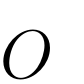
\begin{tikzpicture}
                \path[use as bounding box] (0, 0) rectangle (1em, 1em);
                \draw (0, 0) node {\Huge $O$};
              \end{tikzpicture}
          \\
            & \ddots &
          \\
              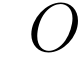
\begin{tikzpicture}
                \path[use as bounding box] (0, 0) rectangle (-1em, -1em);
                \draw (0, 0) node {\Huge $O$};
              \end{tikzpicture}
            & & \vecz_{n}
          \end{genmat}
      &
        \Hat{A} &\defeq \frac{1}{\alpha} Z^{-1} A Z
      \end{align*}
      で $\Hat{A}$ を定めると
      \begin{align*}
        \Hat{A} \vecone
        = \frac{1}{\alpha} Z^{-1} A Z \vecone
        = \frac{1}{\alpha} Z^{-1} A \vecz
        = \frac{1}{\alpha} Z^{-1} \paren{\alpha \vecz}
        = Z^{-1} \vecz
        = \vecone
      \end{align*}
      より $\Hat{A}$ は確率行列である.すなわち,既約な非負正方行列からは確率行列が構成される.
    }
    \thmpar[thm:gershgorin]{Gershgorinの定理}{
      正方行列 $A \in \setMatrix{n}{n}{\setR}$ に対し,$A$ の任意の固有値は
      \begin{align*}
        r_{i} &\defeq \sum_{\scriptrange{j \in \Natleq{n} \setmns \setprn{i}}} \absprn{A_{i j}}
      &
        D_{i} &\defeq \setprnsep{z \in \setC}{\absprn{z - A_{i i}} \leq r_{i}}
      \end{align*}
      で定められる各円板の和集合 $\DS \bigcup \setprnsep{D_{i}}{i \in \Natleq{n}}$ に含まれる.
    }
    \proof{}{
      $A$ の固有値 $\lambda$ とそれに対応する固有ベクトルのひとつ $\vecx$ に対し,各 $i \in \Natleq{n}$ に於いて
      $\DS \sum_{j = 1}^{n} A_{i j} \vecx_{j} = \lambda \vecx_{j}$ である.
      $\DS k \in \argmax_{\scriptrange{j \in \Natleq{n}}} \absprn{\vecx_{j}}$ とすると,
      固有ベクトルの定義より $\vecx \neq \veczero$ であるから $\vecx_{j} \neq 0$ である.
      また,移項により
      $\DS \paren{\lambda - A_{k k}} \vecx_{k}
        = \hspace{-1em}\sum_{\scriptrange{j \in \Natleq{n} \setmns \setprn{k}}}\hspace{-0.75em} A_{k j} \vecx_{j}$%(nonsemantic)
      を得る.この両辺の絶対値をとって
      \begin{align*}
        \absprn{\lambda - A_{k k}} \cdot \absprn{\vecx_{k}}
        = \absprn{\paren{\lambda - A_{k k}} \vecx_{k}}
        &= \absprn{\sum_{\scriptrange{j \in \Natleq{n} \setmns \setprn{k}}}\hspace{-0.75em} A_{k j} \vecx_{j}}%(nonsemantic)
      \\&\leq \sum_{\scriptrange{j \in \Natleq{n} \setmns \setprn{k}}}\hspace{-0.75em} \absprn{A_{k j}} \cdot \absprn{\vecx_{j}}%(nonsemantic)
      \end{align*}
      が成り立ち,したがって
      \begin{align*}
        \absprn{\lambda - A_{k k}}
        &\leq \frac{1}{\absprn{\vecx_{k}}} \sum_{\scriptrange{j \in \Natleq{n} \setmns \setprn{k}}}\hspace{-0.75em}%(nonsemantic)
                \absprn{A_{k j}} \cdot \absprn{\vecx_{j}}
          \holdby{$\vecx_{k} \neq 0$}
      \\&= \sum_{\scriptrange{j \in \Natleq{n} \setmns \setprn{k}}}\hspace{-0.75em}%(nonsemantic)
             \absprn{A_{k j}} \cdot \frac{\absprn{\vecx_{j}}}{\absprn{\vecx_{k}}}
      \\[0.5em]
      &\leq \sum_{\scriptrange{j \in \Natleq{n} \setmns \setprn{k}}}\hspace{-1em} \absprn{A_{k j}}%(nonsemantic)
          \holdby{$k$ の定義}
      \end{align*}
      である.これは $\lambda \in D_{k}$ と同値.ゆえに任意の $A$ の固有値 $\lambda$ に対して
      $\lambda \in D_{k}$ なる $k \in \Natleq{n}$ が存在し,
      すなわち $\DS \lambda \in \bigcup \setprnsep{D_{i}}{i \in \Natleq{n}}$ である.\qed
    }
    \corpar{}{
      任意の確率行列のすべての固有値は絶対値が $1$ 以下である.
    }
    \proof{}{
      $A \in \setMatrix{n}{n}{\setR}$ を確率行列とする.定理~\ref{thm:gershgorin}より,
      各円板 $D_{i}$ の中心 $A_{i i}$ は非負性より $A_{i i} \geq 0$,半径は
      \begin{align*}
        r_{i}
        = \hspace{-0.75em}\sum_{\scriptrange{j \in \Natleq{n} \setmns \setprn{i}}}\hspace{-0.75em} \absprn{A_{i j}}%(nonsemantic)
        &= \hspace{-0.75em}\sum_{\scriptrange{j \in \Natleq{n} \setmns \setprn{i}}}\hspace{-0.75em} A_{i j}%(nonsemantic)
          \holdby{$A > O$}
      \\&= 1 - A_{i i}
          \holdby{$A$ は確率行列なので $A \vecone = \vecone$}
      \end{align*}
      であるから,この $D_{i}$ は複素平面上の単位円板 $S^{1}$ に包まれる(図~\ref{fig:disk-gershgorin}).
      ゆえに $A$ の任意の固有値 $\lambda \in \setC$ に対して
      $\DS \lambda \in \bigcup \setprnsep{D_{i}}{i \in \Natleq{n}} \subseteq S^{1}$ が成り立ち,
      $\absprn{\lambda} \leq 1$ である.\qed
    }
    \begin{figure}[tb]
    \centering
      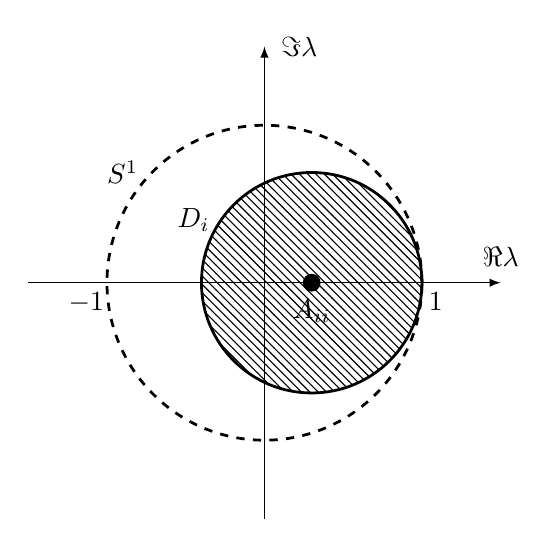
\begin{tikzpicture}[x=2cm,y=2cm]
        \draw[-latex] (0, -1.5) -- (0, 1.5) node[right=0.25em] {$\Im \lambda$};
        \draw[-latex] (-1.5, 0) -- (1.5, 0) node[above=0.25em] {$\Re \lambda$};
        \draw[line width=1pt,dashed] (0, 0) circle[radius=1];
        \fill[pattern=north west lines] (0.3, 0) circle[radius=0.7];
        \draw[line width=1pt] (0.3, 0) circle[radius=0.7];
        \draw[fill=black] (0.3, 0) circle[radius=3pt] node[below=0.25em] {$A_{i i}$};
        \draw (1, 0) node[right=0.5em,below] {$1$};
        \draw (-1, 0) node[left=0.75em,below] {$-1$};
        \draw (-0.45, 0.4) node {$D_{i}$};
        \draw (-0.9, 0.7) node {$S^{1}$};
      \end{tikzpicture}
      \caption{円板 $D_{i i}$ の単位円板 $S^{1}$ による包含}\label{fig:disk-gershgorin}
    \end{figure}
    \thmpar{Birkhoff--von Neumannの定理}{
      任意の二重確率行列は置換行列の凸結合である.
    }
    \proof{}{
      二重確率行列 $A \in \setMatrix{n}{n}{\setR}$ の非零成分の個数 $m$ に関する帰納法による.
      $A \vecone = \vecone$ および $\trsps{\vecone} A = \trsps{\vecone}$ より,各行各列は少なくとも $1$ 個の非零成分をもち,
      したがって $m \geq n$ である.
      \begin{itemize}
      \item $m = n$ のとき,
        $A$ は明らかに置換行列であるから,置換行列の凸結合.
      \item $m > n$ のとき,
        二部グラフ $G = \seqprn{U, V; E}$ を $U \defeq V \defeq \Natleq{n}$,$E \defeq \setprnsep{\seqprn{i, j} \in U \times V}{A_{i j} > 0}$
        で定めると,任意の $X \subseteq U$ に対して
        \begin{align*}
          \card{\app{\Gamma}{X}}
          = \sum_{\scriptrange{j \in \app{\Gamma}{X}}} 1
          &= \sum_{\scriptrange{j \in \app{\Gamma}{X}}} \sum_{i \in U} A_{i j}
            \holdby{$A \vecone = \vecone$}
        \\&= \sum_{i \in U} \sum_{\scriptrange{j \in \app{\Gamma}{X}}} A_{i j}
        \\&\geq \sum_{i \in X} \sum_{\scriptrange{j \in \app{\Gamma}{X}}} A_{i j}
            \holdby{$X \subseteq U$}
        \\&= \sum_{i \in X} \sum_{j \in V} A_{i j}
            \holdby{$E$ の定義より $\forallin{i}{X}{\forallin{j}{V \setmns \app{\Gamma}{X}}{A_{i j} = 0}}$}
        \\&= \sum_{i \in X} 1
            \holdby{$\trsps{\vecone} A = \trsps{\vecone}$}
        \\&= \card{X}
        \end{align*}
        が成り立つ.したがって定理~\ref{thm:hall}:Hallの定理より $G$ に完全マッチング $M \subseteq E$ が存在する.
        この $M$ に対応する行列 $P \in \setMatrix{n}{n}{\setR}$ を
        \begin{align*}
          P_{i j} &\defeq
            \begin{cases}
              1 &\caseif{\seqprn{i, j} \in M}
            \\
              0 &\caseow
            \end{cases}
        \end{align*}
        で定めると,この $P$ は $M$ が完全マッチングであることから明らかに置換行列である.
        ここで $\mu \defeq \min \setprnsep{A_{i j}}{\seqprn{i, j} \in U \times V}$ とおいて
        $\DS A' \defeq \frac{1}{1 - \mu} \paren{A - \mu P}$ とすると,
        $\mu$ の定義より $A' \geq O$ であり,また
        \begin{align*}
          A' \vecone
          &= \frac{1}{1 - \mu} \paren{A \vecone - \mu P \vecone}
          = \frac{1}{1 - \mu} \paren{\vecone - \mu \vecone}
          = \vecone
        \\
          \trsps{\vecone} A'
          &= \frac{1}{1 - \mu} \paren{\trsps{\vecone} A - \mu \trsps{\vecone} P}
          = \frac{1}{1 - \mu} \paren{\trsps{\vecone} - \mu \trsps{\vecone}}
          = \trsps{\vecone}
        \end{align*}
        より $A'$ は二重確率行列.
        この $A'$ は $\mu$ の定義より $A$ よりも非零成分数の真に少ない確率行列であるから,
        帰納法の仮定より $A'$ は置換行列の凸結合であり,
        $A = \paren{1 - \mu} A' + \mu P$ より $A$ も置換行列の凸結合.
      \end{itemize}
      以上より,任意の二重確率行列は置換行列の凸結合である.\qed
    }
\section{整数行列}
  \plainpar{}{
    整数行列はグラフなどの構造から現れ,これを用いてグラフに関する議論を行列に関する議論に帰着することができる.
    しかし,実数一般に於ける基本変形は整数性を保存しない.ここでは整数性を維持した基本変形について考える.
  }
  \subsection{整数基本変形と単模性}
    \defpar{整数列基本変形}{
      整数行列 $A \in \setMatrix{m}{n}{\setZ}$ に対する以下のような操作を\newword{整数列基本変形}と呼ぶ:
      \begin{itemize}
      \item 第 $j \in \Natleq{n}$ 列を $-1$ 倍する
      \item 第 $j \in \Natleq{n}$ 列と第 $k \in \Natleq{n}$ 列を入れ替える
      \item 第 $j \in \Natleq{n}$ 列に第 $k \in \Natleq{n}$ 列の $c \in \setZ$ 倍を加える
      \end{itemize}
    }
    \defpar{単模行列}{
      整数正方行列 $Q \in \setMatrix{n}{n}{\setZ}$ が $\absprn{\det Q} = 1$ を満たすとき,
      $Q$ を\newword{単模行列}あるいは\newword{ユニモジュラ行列}と呼ぶ.
    }
    \lempar[lem:product-preserves-unimodularity]{}{
      単模性は積により保存する.すなわち任意の単模行列 $Q_{1}, Q_{2} \in \setMatrix{n}{n}{\setZ}$ に対して $Q_{1} Q_{2}$ は単模行列である.
    }
    \proof{}{
      $Q_{1}, Q_{2}$ を単模行列とすると
      \begin{align*}
        \absprn{\det \paren{Q_{1} Q_{2}}}
        &= \absprn{\det Q_{1} \cdot \det Q_{2}}
          \holdby{定理~\ref{thm:det-mult-homomorphism}}
      \\&= \absprn{\det Q_{1}} \cdot \absprn{\det Q_{2}}
      = 1
      \end{align*}
      より $Q_{1} Q_{2}$ も単模行列.\qed
    }
    \lempar{}{
      整数正方行列 $Q \in \setMatrix{n}{n}{\setZ}$ に対し,
      $Q$ が単模行列であることと $Q$ が整数正方行列を逆行列にもつことは同値.
    }
    \proof{}{省略.}
    \plainpar{}{
      整数行列 $A$ に整数列基本変形を繰り返し適用することは,或る単模行列 $Q$ を右からかけることに相当する.
      というのも,第 $j$ 列を $-1$ 倍する操作を表す $\app{P}{j}$,第 $j$ 列と第 $k$ 列を交換する操作を表す $\app{Q}{j, k}$,
      第 $j$ 列の $c$ 倍を第 $k$ 列に加える操作を表す $\app{R}{j, k; c}$ \NEEDPICTURE はいずれも単模行列で,
      これらの積も補題~\ref{lem:product-preserves-unimodularity}より単模行列なためである.
    }
    \thmpar{Hermite標準形}{
      $\rank A = m$ なる整数行列 $A \in \setMatrix{m}{n}{\setZ}$ に対し,
      或る置換行列 $P \in \setMatrix{m}{m}{\setZ}$ と単模行列 $\setMatrix{n}{n}{\setZ}$ が存在して
      \begin{align*}
        P A Q &=
          \begin{genmat}{cccc}
            \beta_{1 1} & & &
              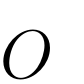
\begin{tikzpicture}
                \path[use as bounding box] (0, 0) -- (1em, 1em);
                \draw (0, 0) node {\Huge $O$};
              \end{tikzpicture}
          \\
            \vdots & \ddots & &
          \\
            \beta_{m 1} & \cdots & \beta_{m m} & 
          \end{genmat}
      \end{align*}
      の形に下三角化でき,しかも
      $\forallin{j}{\Natleq{m}}{\lfland{\beta_{j j} > 0}{\forallin{i}{\Natintvl{j + 1}{m}}{\absprn{\beta_{i j}} < \beta_{i i}}}}$
      を満たす.
    }
    \TODO{証明,ラフに}
    \corpar{}{
      任意の単模行列は列基本変形を表す行列の積.
    }
    \TODO{証明}
  \subsection{行列式因子}
    \defpar{行列式因子}{
      行列 $A$ の $k$ 次小行列式の最大公約数 $\app{g_{k}}{A}$ を,$A$ の $k$ 次の\newword{行列式因子}と呼ぶ.
    }
    \lempar{}{
      行列式因子は,整数列基本変形によって不変である.
    }
    \TODO{行列式因子}
    \TODO{Smith標準形}
\section{線型計画法}
  \subsection{概要}
    \defpar{線型計画問題}{
      線型等式/不等式制約のもとで線型の目的函数を最適化する問題,すなわち
      $A \in \setMatrix{m}{n}{K}$,$\vecb \in \setMatrix{m}{1}{K}$,$\vecc \in \setMatrix{1}{n}{K}$ に対し,
      $A \vecx \leq \vecb$ かつ $\vecx \geq \veczero$ なる $\vecx \in \setMatrix{n}{1}{K}$ で
      $\vecc \vecx$ を最大にするようなものを求める問題を\newword{線型計画問題}と呼び,この問題を
      \begin{align*}
        \text{\parbox[c]{0.5\textwidth}{\Maximize{
          \vecc \vecx
        }{
          A \vecx &\leq \vecb
        | \vecx &\geq \veczero
        }{}}}
        \tag{P}\label{linprob:P}
      \end{align*}
      と表す.この線型計画問題に於いて
      $A \vecx \leq \vecb$ かつ $\vecx \geq \veczero$ なる $\vecx \in \setMatrix{n}{1}{K}$ を\newword{実行可能解}と呼び,
      実行可能解が存在する線型計画問題は\newword{実行可能}であるという.
    }
  \subsection{双対性}
    \plainpar{}{
      線型計画問題~\eqref{linprob:P}の最適解の上界をできるだけタイトに与えようという動機から,
      $A$ の行ベクトルの非負結合で $\vecc$ よりも各成分が大きいものを与えてやることを考える.
      $\vecy A \geq \vecc$ かつ $\vecy \geq \veczero$ なる $\vecy \in \setMatrix{1}{m}{K}$ に対して
      \begin{align*}
        \vecc \vecx \leq \vecy A \vecx &\leq \vecy \vecb
      \end{align*}
      が成り立つことから
      \begin{align*}
        \text{\parbox[c]{0.5\textwidth}{\Maximize{
          \vecy \vecb
        }{
          \vecy A &\geq \vecc
        | \vecy &\geq \veczero
        }{}}}
        \tag{D}\label{linprob:D}
      \end{align*}
      という\eqref{linprob:P}の\newword{双対問題}~\eqref{linprob:D}が生じる.
    }
    \thmpar[thm:weak-duality]{弱双対定理}{
      $\vecx \in \setMatrix{n}{1}{K}$ が\eqref{linprob:P}の実行可能解,
      $\vecy \in \setMatrix{1}{m}{K}$ が\eqref{linprob:D}の実行可能解ならば,
      $\vecc \vecx \leq \vecy \vecb$ が成り立つ.
    }
    \proof{}{
      上記の説明による.\qed
    }
    \thmpar[thm:farkas-lemma]{Farkasの補題}{
      以下が成り立つ:
      \begin{align*}
        \forallin{A}{\setMatrix{m}{n}{K}}{\forallin[3=\hspace{-10em}]{\vecb}{\setMatrix{m}{1}{K} \setmns \setprn{\veczero}}{
          \lflimpleqv{
            \existsin{\vecx}{\setMatrix{n}{1}{K}}{\lfland{A \vecx = \vecb}{\vecx \geq \veczero}}
          }{
            \forallin{\vecy}{\setMatrix{1}{m}{K}}{\lflimpl{\vecy A \geq \veczero}{\vecy \vecb \geq 0}}
          }
        }}
      \end{align*}
    }
    \proof{}{
      \subproof{$\limpl$}{
        $A \vecx = \vecb$ かつ $\vecx \geq \veczero$ なる $\vecx$ をとり,$\vecy A \geq \veczero$ とすると
        $\vecy \vecb = \vecy A \vecx \geq 0$.\qed
      }
      \subproof{$\backlimpl$}{
        $\vecb \in \setprnsep{A \vecx}{\lfland{\vecx \in \setMatrix{n}{1}{K}}{\vecx \geq \veczero}}$,
        すなわち $\vecb$ が $A$ の列ベクトルの非負結合全体のなす凸錐に含まれることを示せばよい.
        仮にこれが成り立たないとすると,$A$ のなす凸錐と $b$ を分離する $m$ 次元超平面 $H$ が存在する.
        図~\ref{fig:H-separates-b-and-A}に概略図を示す.
        このとき,$H$ の法線ベクトルのうち“$A$ 側”に伸びるもののひとつを $\vecy$ とおくと,
        明らかに $\vecy A \geq \veczero$ かつ $\vecy \vecb < 0$ を満たし,仮定に矛盾する.
        ゆえに $\vecb \in \setprnsep{A \vecx}{\lfland{\vecx \in \setMatrix{n}{1}{K}}{\vecx \geq \veczero}}$ が成り立ち,
        したがって $\existsin{\vecx}{\setMatrix{n}{1}{K}}{\lfland{A \vecx = \vecb}{\vecx \geq \veczero}}$ である.\qed
      }
    }
    \begin{figure}[tb]
    \centering
      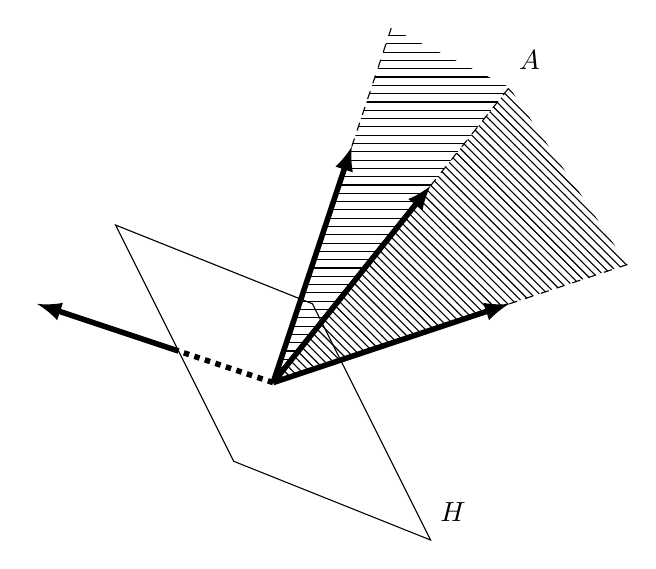
\begin{tikzpicture}
        \draw[dotted, line width=2pt] (0, 0) -- (-1.2, 0.4);
        \draw[-latex, line width=2pt] (-1.2, 0.4) -- (-3, 1) node[above] {$\vecb$};
      %
        \fill[pattern=horizontal lines] (0, 0) -- (1.5, 4.5) -- (3, 3.75) -- cycle;
        \fill[pattern=north west lines] (0, 0) -- (3, 3.75) -- (4.5, 1.5) -- cycle;
      %
        \draw[-latex, line width=2pt] (0, 0) -- (1, 3);
        \draw[-latex, line width=2pt] (0, 0) -- (2, 2.5);
        \draw[-latex, line width=2pt] (0, 0) -- (3, 1);
        \draw[dashed] (1, 3) -- (1.5, 4.5);
        \draw[dashed] (2, 2.5) -- (3, 3.75) node[above=1em,right] {$A$};
        \draw[dashed] (3, 1) -- (4.5, 1.5);
      %
        \draw (-2, 2) -- (-0.5, -1) -- (2, -2) node[above=1em,right] {$H$} -- (0.5, 1) -- cycle;
      \end{tikzpicture}
      \caption{$\vecb$ と $A$ の凸錐を分離する $m$ 次元超平面 $H$ の概略図}\label{fig:H-separates-b-and-A}
    \end{figure}
    \thmpar[thm:expansion-of-farkas-lemma]{}{
      以下が成り立つ:
      \begin{multline*}
        \forallin{A}{\setMatrix{m}{n}{K}}{\forallin[2]{\vecb}{\setcolvec{\setR}{m} \setmns \setprn{\veczero}}{
          \lflimpleqv{
            \existsin{\vecx}{\setcolvec{\setR}{n}}{\lfland{A \vecx \leq \vecb}{\vecx \geq \veczero}}
          }{
            \forallin{\vecy}{\setrowvec{\setR}{m}}{\lflimpl{\lfland{\vecy A \geq \veczero}{\vecy \geq \veczero}}{\vecy \vecb \geq 0}}
          }
        }}
      \end{multline*}
    }
    \proof{}{
      \begin{align*}
        &\existsin{\vecx}{\setcolvec{\setR}{n}}{\lfland{A \vecx \leq \vecb}{\vecx \geq \veczero}}
      \\&\iff
          \existsin{\vecx}{\setcolvec{\setR}{n}}{\existsin{\vecs}{\setcolvec{\setR}{m}}{
            \lfland{\lfland{A \vecx + \vecs = \vecb}{\vecs \geq \veczero}}{\vecx \geq \veczero}
          }}
      \\&\iff
          \existsin{
            \begin{genmat}{@{}c@{}}
              \vecx
            \\\hline
              \vecs
            \end{genmat}
          }{\setcolvec{\setR}{\paren{m + n}}}{
            \lfland{
              {\begin{genmat}{c|c}
                A & I
              \end{genmat}}
              {\begin{genmat}{@{}c@{}}
                \vecx
              \\\hline
                \vecs
              \end{genmat}}
              = \vecb
            }{
              {\begin{genmat}{@{}c@{}}
                \vecx
              \\\hline
                \vecs
              \end{genmat}}
              \geq \veczero
            }
          }
      \\&\iff
          \forallin{\vecy}{\setrowvec{\setR}{m}}{
            \lflimpl{
              \vecy
                {\begin{genmat}{c|c}
                  A & I
                \end{genmat}}
              \geq \veczero
            }{
              \vecy \vecb \geq 0
            }
          }
        \holdby{定理~\ref{thm:farkas-lemma}:Farkasの補題}
      \\&\iff
          \forallin{\vecy}{\setrowvec{\setR}{m}}{
            \lflimpl{
                {\begin{genmat}{c|c}
                  \vecy A & \vecy
                \end{genmat}}
              \geq \veczero
            }{
              \vecy \vecb \geq 0
            }
          }
      \\&\iff
          \forallin{\vecy}{\setrowvec{\setR}{m}}{
            \lflimpl{
              \lfland{
                \vecy \geq \veczero
              }{
                \vecy A \geq \veczero
              }
            }{
              \vecy \vecb \geq 0
            }
          }
      \end{align*}
      \qed
    }
    \thmpar[thm:strong-duality]{強双対定理}{
      主問題~\eqref{linprob:P}とその双対問題~\eqref{linprob:D}が共に実行可能であるとき,
      それぞれに最適解 $\vecxopt$,$\vecyopt$ が存在して $\vecc \vecxopt = \vecyopt \vecb$ を満たす.
    }
    \proof{}{
      定理~\ref{thm:weak-duality}:弱双対定理より,
      或る実行可能解 $\vecx$,$\vecy$ が存在して $\vecc \vecx \geq \vecy \vecb$ を満たすこと,すなわち
      \begin{align*}
        \existsin{\vecx}{\setcolvec{\setR}{n}}{\existsin{\vecy}{\setrowvec{\setR}{m}}{
          \lfland{
            \lfland{\lfland{A \vecx \leq \vecb}{\vecx \geq \veczero}}{\lfland{\vecy A \geq \vecc}{\vecy \geq \veczero}}
          }{
            \vecc \vecx \geq \vecy \vecb
          }
        }}
      \end{align*}
      を示せばよい.さらにこれは
      \begin{align*}
        &\existsin{\vecx}{\setcolvec{\setR}{n}}{\existsin{\vecy}{\setrowvec{\setR}{m}}{
          \lfland{
            \lfland{\lfland{A \vecx \leq \vecb}{\vecx \geq \veczero}}{\lfland{\vecy A \geq \vecc}{\vecy \geq \veczero}}
          }{
            \vecc \vecx \geq \vecy \vecb
          }
        }}
      \\&\iff
          \existsin{
            {\begin{genmat}{@{}c@{}}
              \vecx
            \\\hline
              \trsps{\vecy}
            \end{genmat}}
          }{\setcolvec{\setR}{\paren{m + n}}}{
            \lfland{
              {\begin{genmat}{c|c}
                A & O
              \\\hline
                O & -\trsps{A}
              \\\hline
                - \vecc & \trsps{\vecb}
              \end{genmat}}
              {\begin{genmat}{@{}c@{}}
                \vecx
              \\\hline
                \trsps{\vecy}
              \end{genmat}}
              \leq
              {\begin{genmat}{@{}c@{}}
                \vecb
              \\\hline
                - \trsps{\vecc}
              \\\hline
                0
              \end{genmat}}
            }{
            {\begin{genmat}{@{}c@{}}
              \vecx
            \\\hline
              \trsps{\vecy}
            \end{genmat}}
            \geq \veczero
            }
          }
      \\&\iff
          \forallin{
            {\begin{genmat}{c|c|c}
              \vecu & \trsps{\vecv} & \theta
            \end{genmat}}
          }{\setrowvec{\setR}{\paren{m + n + 1}}}{
            \lflimpl{
              \lfland{
                {\begin{genmat}{c|c|c}
                  \vecu & \trsps{\vecv} & \theta
                \end{genmat}}
                \geq \veczero
              }{
                {\begin{genmat}{c|c|c}
                  \vecu & \trsps{\vecv} & \theta
                \end{genmat}}
                {\begin{genmat}{c|c}
                  A & O
                \\\hline
                  O & -\trsps{A}
                \\\hline
                  - \vecc & \trsps{\vecb}
                \end{genmat}}
                \geq \veczero
              }
            \midbreak\midtab\hspace{10em}%(nonsemantic)
            }{
              {\begin{genmat}{c|c|c}
                \vecu & \trsps{\vecv} & \theta
              \end{genmat}}
              {\begin{genmat}{@{}c@{}}
                \vecb
              \\\hline
                - \trsps{\vecc}
              \\\hline
                0
              \end{genmat}}
              \geq 0
            }
          }
            \holdby{定理~\ref{thm:expansion-of-farkas-lemma}}
    \\&\iff
        \forallin{\theta}{\setR}{\forallin{\vecu}{\setrowvec{\setR}{m}}{\forallin[3=\hspace{4em}]{\vecv}{\setcolvec{\setR}{n}}{
          \lflimpl{
            \lfland{
              \lfland{\lfland{\vecu \geq \veczero}{\vecv \geq \veczero}}{\theta \geq 0}
            }{
              \lfland{\vecu A \geq \theta \vecc}{A \vecv \leq \theta \vecb}
            }
          }{
            \vecc \vecv \leq \vecu \vecb
          }
        }}}
      \end{align*}
      と同値変形できるので,この最後の命題を示せばよい.
      \begin{itemize}
      \item $\theta = 0$ のとき,
        仮定より\eqref{linprob:P}と\eqref{linprob:D}は共に実行可能であるからそれぞれに実行可能解 $\vecx$,$\vecy$ が存在し,
        これらをひとつずつとって
        \begin{align*}
          \vecc \vecv
          &\leq \vecy A \vecv
            \holdby{$\vecy A \geq \vecc$ および $\vecv \geq \veczero$}
        \\&\leq \veczero
            \holdby{$\vecy \geq \veczero$ および $A \vecv \leq \veczero$}
        \\&\leq \vecu A \vecx
            \holdby{$\vecu A \geq \veczero$ および $\vecx \geq \veczero$}
        \\&\leq \vecu \vecb
            \holdby{$\vecu \geq \veczero$ および $A \vecx \leq \vecb$}
        \end{align*}
        であるから $\vecc \vecv \leq \vecu \vecb$ が成り立つ.
      \item $\theta > 0$ のとき,
        $\vecu \geq \veczero$ かつ $\vecu A \geq \theta \vecc$ なる $\vecu \in \setrowvec{\setR}{m}$,および
        $\vecv \geq \veczero$ かつ $A \vecv \leq \theta \vecb$ なる $\vecv \in \setcolvec{\setR}{n}$ に対して
        $\DS \vecp \defeq \frac{1}{\theta} \vecu$,$\DS \vecq \defeq \frac{1}{\theta} \vecv$ とすると,
        $\vecp \geq \veczero$,$\vecq \geq \veczero$,および $\vecp A \geq \vecc$,$A \vecq \leq \vecb$ が成り立つ.
        すなわち,$\vecq$ と $\vecp$ はそれぞれ主問題~\eqref{linprob:P}とその双対問題~\eqref{linprob:D}の実行可能解である.
        したがって定理~\ref{thm:weak-duality}:弱双対定理より $\vecc \vecq \leq \vecp \vecb$ が成り立ち,
        これの両辺に $\theta$ を乗じて $\vecc \vecv \leq \vecu \vecb$ を得る.
      \end{itemize}
      以上より,或る実行可能解 $\vecx$,$\vecy$ が存在して $\vecc \vecx \geq \vecy \vecb$ を満たす.\qed
    }
    \thmpar{相補最適性}{
      主問題~\eqref{linprob:P}と双対問題~\eqref{linprob:D}の実行可能解 $\vecx$,$\vecy$ に対し,
      $\vecx$ と $\vecy$ がそれぞれ\eqref{linprob:P}と\eqref{linprob:D}の最適解であることと
      \begin{align*}
        \lfland{
          \forallin{j}{\Natleq{n}}{\lflimpl{\vecx_{j} > 0}{\paren{\vecy A}_{j} = \vecc_{j}}}
        }{
          \forallin{i}{\Natleq{m}}{\lflimpl{\vecy_{i} > 0}{\paren{A \vecx}_{i} = \vecb_{i}}}
        }
      \end{align*}
      が成り立つことは同値.
    }
    \proof{}{
      \subproof{$\limpl$}{
        $\vecx$ と $\vecy$ がそれぞれ\eqref{linprob:P}と\eqref{linprob:D}の最適解であるとすると,
        定理~\ref{thm:strong-duality}:強双対定理より $\vecc \vecx = \vecy A \vecx = \vecy \vecb$ が成り立つ.
        したがって $\paren{\vecy A - \vecc} \vecx = 0$ であるが,
        $\vecy A - \vecc \geq \veczero$ かつ $\vecx \geq \veczero$ より
        各 $j \in \Natleq{n}$ に対して $\paren{\vecy A - \vecc}_{j} \geq 0$ かつ $\vecx_{j} \geq 0$ である.
        よって $\vecx_{j} > 0$ とすると $\paren{\vecy A - \vecc}_{j} = 0$,すなわち $\paren{\vecy A}_{j} = \vecc_{j}$.
        同様に $\vecy \paren{A \vecx - \vecb} = 0$ からも $\vecy_{i} > 0$ ならば $\paren{A \vecx}_{i} = \vecb_{i}$ が成り立つ.\qed
      }
    }
  \subsection{行列ゲーム}
    \plainpar{}{
      対戦者 X と Y がとれる手の有限集合をそれぞれ $U$,$V$ とし,自分の選択した手 $i \in U$ と相手の選択した手 $j \in V$ に依存して
      X の利得 $A_{i j} \in \setR$ が決まるとする.このとき Y の利得は $-A_{i j}$ とする.すなわち\newword{零和}である.
      手を選ぶ際に,相手の選んだ手を見ることはできず,双方が選んで初めて照合する.
      ここでは X と Y が共に一定の確率の割り振りで各回独立に手を選ぶ戦略である\newword{混合戦略}を考える.
      X が手 $i \in U$ を選ぶ確率を $\vecp_{i}$,Y が手 $j \in V$ を選ぶ確率を $\vecq_{j}$ として,
      $\vecp \geq \trsps{\veczero}$,$\vecp \vecone = 1$,$\vecq \geq \veczero$,$\trsps{\vecone} \vecq = 1$
      なるベクトル $\vecp$,$\vecq$ を考える.
      この戦略の下で,X の利得の期待値は $\vecp A \vecq$ である.X にとってはこれを大きくすることが望ましいわけである.
      X と Y のとれる混合戦略全体からなる集合をそれぞれ
      \begin{align*}
        P &\defeq \setprnsep{\vecp \in \setrowvec{\setR}{m}}{\lfland{\vecp \geq \trsps{\veczero}}{\vecp \vecone = 1}}
      \\
        Q &\defeq \setprnsep{\vecq \in \setcolvec{\setR}{n}}{\lfland{\vecq \geq \veczero}{\trsps{\vecone} \vecq = 1}}
      \end{align*}
      とおいておく.
    }
    \thmpar{鞍点定理}{
      $A \in \setMatrix{m}{n}{\setR}$ に対して,以下が成り立つ:
      \begin{align*}
        \max \setprnsep{\min \setprnsep{\vecp A \vecq}{\vecq \in Q}}{\vecp \in P}
        &=
        \min \setprnsep{\max \setprnsep{\vecp A \vecq}{\vecp \in P}}{\vecq \in Q}
      \end{align*}
    }
    \proof{}{
      $\vecp$ を固定すると $\min \setprnsep{\vecp A \vecq}{\vecq \in Q}$ は $\vecq$ に関する線型計画問題:
      \begin{align*}
          \text{\parbox{10em}{
            \Minimize{\paren{\vecp A} \vecq}{
              \trsps{\vecone} \vecq &= 1
            | \vecq &\geq \veczero
            }{}}}
        &\quad\cong\quad
          \text{\parbox{10em}{\Minimize{\paren{\vecp A} \vecq
          }{
            \trsps{\vecone} \vecq &\leq 1
          | \trsps{\vecone} \vecq &\geq 1
          | \vecq &\geq \veczero
          }{}}}
      \\&\quad\cong\quad
          \text{\parbox{18em}{\Minimize{
            \paren{\vecp A} \vecq
          }{
            \begin{genmat}{c}
              \expandH{\trsps{\vecone}}
            \\\hline
              \expandH{{-}\trsps{\vecone}}
            \end{genmat}
            \vecq
          &\leq
            \begin{genmat}{@{}c@{}}
              1
            \\
              -1
            \end{genmat}
          | \vecq &\geq \veczero
          }{}}}
      \end{align*}
      と看なせる.したがって定理~\ref{thm:strong-duality}:強双対定理より,双対問題:
      \begin{align*}
          \text{\parbox{18em}{\Maximize{
            \vecz
            \begin{genmat}{@{}c@{}}
              1
            \\
              -1
            \end{genmat}
          }{
            \vecz
            \begin{genmat}{c}
              \expandH{\trsps{\vecone}}
            \\\hline
              \expandH{{-}\trsps{\vecone}}
            \end{genmat}
            &\leq \vecp A
          | \vecz &\geq \veczero
          }{}}}
        &\quad\cong\quad
          \text{\parbox{15em}{\Maximize{
            z_{1} - z_{2}
          }{
            \paren{z_{1} - z_{2}} \trsps{\vecone} &\leq \vecp A
          | z_{1} &\geq 0
          | z_{2} &\geq 0
          }{}}}
      \\&\quad\cong\quad
          \text{\parbox{10em}{\Maximize{
            z
          }{
            z \trsps{\vecone} &\leq \vecp A
          }{}}}
      \end{align*}
      を考えると
      $\min \setprnsep{\vecp A \vecq}{\vecq \in Q} = \max \setprnsep{z \in \setR}{z \trsps{\vecone} \leq \vecp A}$
      が成り立つ.よって
      \begin{align}
        \max \setprnsep{\min \setprnsep{\vecp A \vecq}{\vecq \in Q}}{\vecp \in P}
        &= \max \setprnsep{\max \setprnsep{z \in \setR}{z \trsps{\vecone} \leq \vecp A}}{\vecp \in P}
          \notag
      \\&= \max \setprnsep{z \in \setR}{\lfland{\vecp \in P}{z \trsps{\vecone} - \vecp A \leq \trsps{\veczero}}}
          \label{eq:saddle-point-1}
      \end{align}
      である.さて,再び $\max \setprnsep{z \in \setR}{\lfland{\vecp \in P}{z \trsps{\vecone} - \vecp A \leq \trsps{\veczero}}}$ は
      線型計画問題:
      \begin{align*}
          &
          \text{\parbox[c]{14em}{\Maximize{
            z
          }{
            z \trsps{\vecone} - \vecp A &\leq \trsps{\veczero}
          | \vecp \vecone &= 1
          | \vecp &\geq \trsps{\veczero}
          }{}}}
        \quad\cong\quad
          \text{\parbox[c]{24em}{\Maximize{
            z_{1} - z_{2}
          }{
            \begin{genmat}{@{}cc@{}}
              z_{1} & z_{2}
            \end{genmat}
            \begin{genmat}{c}
              \expandH{\trsps{\vecone}}
            \\\hline
              \expandH{{-}\trsps{\vecone}}
            \end{genmat}
            - \vecp A &\leq \trsps{\veczero}
          | \vecp
            \begin{genmat}{@{}c|c@{}}
              \expandV{\vecone} & \expandV{{-}\vecone}
            \end{genmat}
             &\leq
             \begin{genmat}{@{}cc@{}}
               1 & -1
             \end{genmat}
          | z_{1} &\geq 0
          | z_{2} &\geq 0
          | \vecp &\geq \trsps{\veczero}
        }{}}}
      \\&\quad\cong\quad
          \text{\parbox[c]{24em}{\Maximize{
            \begin{genmat}{@{}cc|c}
              z_{1} & z_{2} & \expandH{\vecp}
            \end{genmat}
            \begin{genmat}{@{}c@{}}
              1
            \\
              -1
            \\\hline
              \expandV{\veczero}
            \end{genmat}
          }{
            \begin{genmat}{@{}cc|c}
              z_{1} & z_{2} & \expandH{\vecp}
            \end{genmat}
            \begin{genmat}{c|c|c}
              0 & 0 & \expandH{\trsps{\vecone}}
            \\\hline
              0 & 0 & \expandH{{-}\trsps{\vecone}}
            \\\hline
              \vecone & -\vecone & \expandHV{{-}A}
            \end{genmat}
            &\leq
            \begin{genmat}{@{}cc|c}
              1 & -1 & \expandH{\trsps{\veczero}}
            \end{genmat}
          | \begin{genmat}{@{}cc|c}
              z_{1} & z_{2} & \expandH{\vecp}
            \end{genmat}
            &\geq \trsps{\veczero}
        }{}}}
      \end{align*}
      と看なせるから,これの双対問題:
      \begin{align*}
        &
          \text{\parbox[c]{23em}{\Minimize{
            \begin{genmat}{@{}cc|c}
              1 & -1 & \expandH{\trsps{\veczero}}
            \end{genmat}
            \begin{genmat}{@{}c@{}}
              w_{1}
            \\
              w_{2}
            \\\hline
              \expandV{\vecq}
            \end{genmat}
          }{
            \begin{genmat}{c|c|c}
              0 & 0 & \expandH{\trsps{\vecone}}
            \\\hline
              0 & 0 & \expandH{{-}\trsps{\vecone}}
            \\\hline
              \vecone & {-}\vecone & \expandHV{{-}A}
            \end{genmat}
            \begin{genmat}{@{}c@{}}
              w_{1}
            \\
              w_{2}
            \\\hline
              \expandV{\vecq}
            \end{genmat}
            &\leq
            \begin{genmat}{@{}c@{}}
              1
            \\
              -1
            \\\hline
              \expandV{\veczero}
            \end{genmat}
          }{}}}
      \\&\quad\cong\quad
          \text{\parbox[c]{18em}{\Minimize{
            w_{1} - w_{2}
          }{
            \trsps{\vecone} \vecq &\leq 1
          | -\trsps{\vecone} \vecq &\leq -1
          | w_{1} \vecone - w_{2} \vecone - A \vecq &\leq \veczero
          | w_{1} &\geq 0
          | w_{2} &\geq 0
          | \vecq &\geq \veczero
          }{}}}
        \quad\cong\quad
          \text{\parbox[c]{14em}{\Minimize{
            w
          }{
            \trsps{\vecone} \vecq =\leq 1
          | w \vecone - A \vecq &\leq \veczero
          | \vecq &\geq \veczero
          }{}}}
      \end{align*}
      に変形でき,
      \begin{align}
        \max \setprnsep{z \in \setR}{\lfland{\vecp \in P}{z \trsps{\vecone} - \vecp A \leq \trsps{\veczero}}}
        &= \min \setprnsep{w \in \setR}{\lfland{\vecq \in Q}{w \vecone - A \vecq \leq \veczero}}
          \notag
      \\&= \min \setprnsep{\setprnsep{w \in \setR}{w \vecone - A \vecq \leq \veczero}}{\vecq \in Q}
          \label{eq:saddle-point-2}
      \end{align}
      が成り立つ.ここでさらに $\vecq$ を固定した下で $\min \setprnsep{w \in \setR}{w \vecone - A \vecq \leq \veczero}$ は線型計画問題:
      \begin{align*}
          \text{\parbox[c]{11em}{\Minimize{
            w
          }{
            w \vecone &\leq A \vecq
          }{}}}
        &\quad\cong\quad
          \text{\parbox[c]{14em}{\Minimize{
            w_{1} - w_{2}
          }{
            w_{1} \vecone - w_{2} \vecone &\leq A \vecq
          }{}}}
      \\&\quad\cong\quad
          \text{\parbox[c]{10em}{\Minimize{
            \begin{genmat}{@{}cc@{}}
              1 & -1
            \end{genmat}
            \begin{genmat}{@{}c@{}}
              w_{1}
            \\
              w_{2}
            \end{genmat}
          }{
            \begin{genmat}{c|c}
              \expandV{\vecone} & \expandV{{-}\vecone}
            \end{genmat}
            &\leq A \vecq
          |
            \begin{genmat}{@{}c@{}}
              w_{1}
            \\
              w_{2}
            \end{genmat}
            &\geq \veczero
          }{}}}
      \end{align*}
      と看なせるから,これの双対問題:
      \begin{align*}
          \text{\parbox[c]{18em}{\Maximize{
            \vecp \paren{A \vecq}
          }{
            \vecp
            \begin{genmat}{@{}c|c@{}}
              \expandV{\vecone} & \expandV{{-}\vecone}
            \end{genmat}
            &\leq
            \begin{genmat}{@{}cc@{}}
              1 & -1
            \end{genmat}
          | \vecp &\geq \trsps{\veczero}
          }{}}}
        &\quad\cong\quad
          \text{\parbox[c]{10em}{\Maximize{
            \vecp A \vecq
          }{
            \vecp \vecone &= 1
          | \vecp &\geq \trsps{\veczero}
          }{}}}
      \end{align*}
      へと変形でき,したがって
      \begin{align}
        \min \setprnsep{w \in \setR}{w \vecone - A \vecq \leq \veczero}
        &= \max \setprnsep{\vecp A \vecq}{\vecp \in P}
        \label{eq:saddle-point-3}
      \end{align}
      が成り立つ.以上の\eqref{eq:saddle-point-1},\eqref{eq:saddle-point-2},\eqref{eq:saddle-point-3}より
      \begin{align*}
        \max \setprnsep{\min \setprnsep{\vecp A \vecq}{\vecq \in Q}}{\vecp \in P}
        &=
        \min \setprnsep{\max \setprnsep{\vecp A \vecq}{\vecp \in P}}{\vecq \in Q}
      \end{align*}
      である.\qed
    }
\section{線型制御システムの可制御系}
  \subsection{行列の指数函数}
    \defpar{行列の指数函数}{
      正方行列 $A$ に対して
      $\DS \npe^{A} \defeq \sum_{k = 1}^{\infty} \frac{1}{k !} A^{k}$
      とする.
    }
    \plainpar{}{
      $A$ と $A$ のJordan標準形 $A' = S^{-1} A S$ に対して
      \begin{align*}
        \npe^{A}
        &= \sum_{k = 1}^{\infty} \frac{1}{k !} \paren{S A' S^{-1}}^{k}
        = \sum_{k = 1}^{\infty} \frac{1}{k !} \paren{S \paren{A'}^{k} S^{-1}}
        = S \paren{\sum_{k = 1}^{\infty} \frac{1}{k !} \paren{A'}^{k}} S^{-1}
        = S \npe^{A'} S^{-1}
      \end{align*}
      である.
    }
    \TODO{Jordan細胞の $n$ 乗}
    \defpar{安定性}{
      正方行列 $A \in \setMatrix{n}{n}{\setR}$ のすべての固有値の実部が負であるとき,$A$ は\newword{安定}であるという.
    }
    \thmpar{Lyapunov不等式}{
      正方行列 $A \in \setMatrix{n}{n}{\setR}$ に対し,$A$ が安定であることと,
      或る正定値対称行列 $Y \in \setMatrix{n}{n}{\setR}$ が存在して $Y A + \trsps{A} Y$ を負定値対称にすることは同値.
    }
    \proof{}{
      \subproof{$\backlimpl$}{
        $\lambda \in \setC$ を $A$ の固有値とし,$\vecv \in \setcolvec{\setC}{n} \setmns \setprn{\veczero}$ を
        $\lambda$ に対応する固有ベクトルのひとつとすると $A \vecv = \lambda \vecv$ であり,
        これの両辺の共軛転置をとって $\conjtrsps{\vecv} \trsps{A} = \conj{\lambda} \conjtrsps{\vecv}$
        である.このとき,仮定の $Y$ をとると
        \begin{align*}
          0
          &> \conjtrsps{\vecv} \paren{Y A + \trsps{A} Y} \vecv
            \holdby{$Y A + \trsps{A} Y$ は不定値}
        \\&= \conjtrsps{\vecv} Y A \vecv + \conjtrsps{\vecv} \trsps{A} Y \vecv
        \\&= \conjtrsps{\vecv} Y \paren{\lambda \vecv} + \paren{\conj{\lambda} \conjtrsps{\vecv}} Y \vecv
        \\&= \paren{\lambda + \conj{\lambda}} \conjtrsps{\vecv} Y \vecv
        \end{align*}
        より $\paren{\lambda + \conj{\lambda}} \conjtrsps{\vecv} Y \vecv < 0$ であるが,
        $Y$ は仮定より正定値であり $\vecv \neq \veczero$ であるから $\conjtrsps{\vecv} Y \vecv > 0$,
        したがって $2 \Re \lambda = \lambda + \conj{\lambda} < 0$.
        ゆえに $\Re \lambda < 0$ であり,$\lambda$ は任意であったから $A$ は安定.\qed
      }
      \subproof{$\limpl$}{
        $A$ を安定な行列とする.正定値対称行列のひとつ $Q \in \setMatrix{n}{n}{\setR}$ を任意にとって
        $\DS Y \defeq \int_{0}^{+\infty} \npe^{t \trsps{A}} Q \npe^{A t} \ordd t$ とおくと
        \begin{align*}
          Y A + \trsps{A} Y
          &= \int_{0}^{+\infty} \dif{}{t}\paren{\npe^{t \trsps{A}} Q \npe^{t A}} \ordd t
            \holdby{成分ごとのいわゆる部分積分}
        \\&= \sqbracket{\npe^{t \trsps{A}} Q \npe^{t A}}_{t = 0}^{+\infty}
          = 0 - I Q I
          = -Q
        \end{align*}
        より $Y A + \trsps{A} Y$ は負定値対称.\qed
      }
    }
    \defpar{Sylvester方程式}{
      行列 $A \in \setMatrix{m}{m}{\setR}$,$B \in \setMatrix{n}{n}{\setR}$,$C \in \setMatrix{m}{n}{\setR}$
      を係数とする,$X \in \setMatrix{m}{n}{\setR}$ に関する方程式
      \begin{align*}
        A X - X \trsps{B} = C
      \end{align*}
      を\newword{Sylvester方程式}と呼ぶ.
    }
    \plainpar{}{
      Sylvester方程式は,制約が高々 $m n$ 個,変数が $m n$ 個なので,制約がすべて“互いに独立”であれば解けることが期待される.
      $X$ と $C$ を
      \begin{align*}
        \vecx &\defeq
          \begin{genmat}{@{}c@{}}
            \expandV{\colvec{X}{1}}
          \\\hline
            \vdots
          \\\hline
            \expandV{\colvec{X}{n}}
          \end{genmat}
      &
        \vecc &\defeq
          \begin{genmat}{@{}c@{}}
            \expandV{\colvec{C}{1}}
          \\\hline
            \vdots
          \\\hline
            \expandV{\colvec{C}{n}}
          \end{genmat}
      \end{align*}
      という成分をすべて縦に並べた形に書き直すと,Sylvester方程式はこれらを使って
      \begin{align*}
        \paren{I_{n} \otimes A - B \otimes I_{m}} \vecx &= \vecc
      \end{align*}
      と同値変形できる.ここで $\otimes$ はKronecker積:
      \begin{align*}
        S \otimes T &\defeq
          \begin{genmat}{c|c|c}
            S_{1 1} T & \cdots & S_{1 n} T
          \\\hline
            \vdots & \ddots & \vdots
          \\\hline
            S_{n 1} T & \cdots & S_{n n} T
          \end{genmat}
      \end{align*}
      である.ここでは具体的には
      \begin{align*}
        I_{n} \otimes A
        &=
          \begin{genmat}{cccc}
            \multicolumn{1}{c|}{A} & & &
              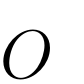
\begin{tikzpicture}
                \path[use as bounding box] (0, 0) -- (1em, 1em);
                \draw (0, 0) node {\Huge $O$};
              \end{tikzpicture}
          \\\cline{1-2}
            & \multicolumn{1}{|c|}{A} & &
          \\\cline{2-2}
             & & \ddots &
          \\\cline{4-4}
              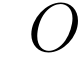
\begin{tikzpicture}
                \path[use as bounding box] (0, 0) -- (-1em, -1em);
                \draw (0, 0) node {\Huge $O$};
              \end{tikzpicture}
            & & & \multicolumn{1}{|c}{A}
          \end{genmat}
      &
        B \otimes I_{m}
        &=
          \begin{genmat}{c|c|c}
            B_{1 1} I_{m} & \cdots & B_{1 n} I_{m}
          \\\hline
            \vdots & \ddots & \vdots
          \\\hline
            B_{n 1} I_{m} & \cdots & B_{n n} I_{m}
          \end{genmat}
      \end{align*}
      となる.
      これにより $D \defeq I_{n} \otimes A - B \otimes I_{m}$ とおくことにより $D \vecx = \vecc$ という普通の線型方程式に帰着されたので,
      $D$ が正則であるときに $\vecx = D^{-1} \vecc$ と過不足なく求められる.では $D$ はいかなる時に正則かということを考える.
      $A$ の固有値 $\lambda$ とそれに対応する固有ベクトルのひとつを $\vecu$,および $B$ の固有値 $\mu$ とそれに対応する固有ベクトルのひとつを $\vecv$ とすると,
      \begin{align*}
        \paren{I_{n} \otimes A} \paren{\vecv \otimes \vecu}
        &=
          \begin{genmat}{ccc}
            \multicolumn{1}{c|}{A} & &
              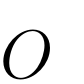
\begin{tikzpicture}
                \path[use as bounding box] (0, 0) -- (1em, 1em);
                \draw (0, 0) node {\Huge $O$};
              \end{tikzpicture}
          \\\cline{1-1}
             & \ddots &
          \\\cline{3-3}
              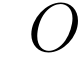
\begin{tikzpicture}
                \path[use as bounding box] (0, 0) -- (-1em, -1em);
                \draw (0, 0) node {\Huge $O$};
              \end{tikzpicture}
            & & \multicolumn{1}{|c}{A}
          \end{genmat}
          \begin{genmat}{@{}c@{}}
            \vecv_{1} \vecu
          \\\hline
            \vdots
          \\\hline
            \vecv_{n} \vecu
          \end{genmat}
        =
          \begin{genmat}{@{}c@{}}
            A \paren{\vecv_{1} \vecu}
          \\\hline
            \vdots
          \\\hline
            A \paren{\vecv_{n} \vecu}
          \end{genmat}
        =
          \begin{genmat}{@{}c@{}}
            \vecv_{1} \lambda \vecu
          \\\hline
            \vdots
          \\\hline
            \vecv_{n} \lambda \vecu
          \end{genmat}
        =
          \lambda \paren{\vecv \otimes \vecu}
      \end{align*}
      が成り立ち,一方
      \begin{align*}
        \paren{B \otimes I_{m}} \paren{\vecv \otimes \vecu}
        &=
          \begin{genmat}{c@{}c@{}c|c|c@{}c@{}c}
            B_{1 1} & & & & B_{1 n} & &
          \\
            & \ddots & & \expandH{\cdots} & & \ddots &
          \\
            & & B_{1 1} & & & & B_{1 n}
          \\\hline
            & \expandV{\vdots} & & \ddots & & \vdots &
          \\\hline
            B_{n 1} & & & & B_{n n} & &
          \\
            & \ddots & & \expandH{\cdots} & & \ddots &
          \\
            & & B_{n 1} & & & & B_{n n}
          \end{genmat}
          \begin{genmat}{@{}c@{}}
            \vecv_{1} \vecu_{1}
          \\
            \vdots
          \\
            \vecv_{1} \vecu_{m}
          \\\hline
            \expandV{\vdots}
          \\\hline
            \vecv_{n} \vecu_{1}
          \\
            \vdots
          \\
            \vecv_{n} \vecu_{m}
          \end{genmat}
        =
          \begin{genmat}{@{}c@{}}
            \sum_{i = 1}^{n} B_{1 i} \vecv_{i} \vecu_{1}
          \\
            \vdots
          \\
            \sum_{i = 1}^{n} B_{n i} \vecv_{i} \vecu_{m}
          \\\hline
            \expandV{\vdots}
          \\\hline
            \sum_{i = 1}^{n} B_{1 i} \vecv_{i} \vecu_{1}
          \\
            \vdots
          \\
            \sum_{i = 1}^{n} B_{n i} \vecv_{i} \vecu_{m}
          \end{genmat}
      \\&=
          \begin{genmat}{@{}c@{}}
            \paren{B \vecv}_{1} \vecu_{1}
          \\
            \vdots
          \\
            \paren{B \vecv}_{n} \vecu_{m}
          \\\hline
            \expandV{\vdots}
          \\\hline
            \paren{B \vecv}_{1} \vecu_{1}
          \\
            \vdots
          \\
            \paren{B \vecv}_{n} \vecu_{m}
          \end{genmat}
        =
          \begin{genmat}{@{}c@{}}
            \paren{\mu \vecv}_{1} \vecu_{1}
          \\
            \vdots
          \\
            \paren{\mu \vecv}_{n} \vecu_{m}
          \\\hline
            \expandV{\vdots}
          \\\hline
            \paren{\mu \vecv}_{1} \vecu_{1}
          \\
            \vdots
          \\
            \paren{\mu \vecv}_{n} \vecu_{m}
          \end{genmat}
        =
          \mu \paren{\vecv \otimes \vecu}
      \end{align*}
      も成り立つから
      \begin{align*}
        D \paren{\vecv \otimes \vecu}
        = \paren{I_{n} \otimes A - B \otimes I_{m}} \paren{\vecv \otimes \vecu}
        &= \paren{\lambda - \mu} \paren{\vecv \otimes \vecu}
      \end{align*}
      であり,$\lambda - \mu$ は $D$ の固有値である.
    }
  \subsection{線型制御システム}
    \plainpar{}{
      行列 $A \in \setMatrix{n}{n}{\setR}$ と行列 $B \in \setMatrix{n}{r}{\setR}$ を係数とする,
      \newword{状態} $\vecx \in \setcolvec{\setR}{n}$ と \newword{入力} $\vecu \in \setcolvec{\setR}{r}$ に関する微分方程式
      \begin{align}
        \dif{}{t}\vecx &= A \vecx + B \vecu
        \label{eq:control-main}
      \end{align}
      を\newword{線型制御システム}と呼ぶ.このような微分方程式が成立しているもとで,状態 $\vecx$ を望み通りに制御するためには
      どのような入力 $\vecu$ を与えればよいか,ということが線型制御システムについて思案する動機である.
    }
    \defpar{可制御性}{
      行列 $A \in \setMatrix{n}{n}{\setR}$,行列 $B \in \setMatrix{n}{r}{\setR}$ に対し,
      \begin{align}
        T^{-1} A T
        &=
        \begin{genmat}{c|c}
          A^{(1 1)} & A^{(1 2)}
        \\\hline
          O & A^{(2 2)}
        \end{genmat}
      &
        T^{-1} B
        &=
        \begin{genmat}{c}
          B^{(1)}
        \\\hline
          O
        \end{genmat}
        \label{eq:uncontrollable}
      \end{align}
      の形を満たすような正則行列 $T \in \setMatrix{n}{n}{\setR}$ が存在しないとき,
      $\seqprn{A, B}$ は\newword{可制御}であるという.
    }
    \plainpar{}{
      可制御でない場合はどのような状態かというと,\eqref{eq:uncontrollable}を満たすような正則行列 $T$ が存在するのでこれをとり,
      $\vecp \defeq T^{-1} \vecx$,$\vecv \defeq T^{-1} \vecu$ と変数をおき直すと
      \begin{align*}
        \dif{}{t}\vecp &= \paren{T^{-1} A T} \vecp + \paren{T^{-1} B} \vecv
      \end{align*}
      すなわち
      \begin{align*}
        \dif{}{t}
        \begin{genmat}{@{}c@{}}
          \vecp^{(1)}
        \\\hline
          \vecp^{(2)}
        \end{genmat}
        &=
          \begin{genmat}{c|c}
            A^{(1 1)} & A^{(1 2)}
          \\\hline
            O & A^{(2 2)}
          \end{genmat}
          \begin{genmat}{@{}c@{}}
            \vecp^{(1)}
          \\\hline
            \vecp^{(2)}
          \end{genmat}
          +
          \begin{genmat}{c}
            B^{(1)}
          \\\hline
            O
          \end{genmat}
          \vecv
        =
          \begin{genmat}{c}
            A^{(1 1)} \vecp^{(1)} + A^{(12)} \vecp^{(2)} + B^{(1)} \vecv
          \\\hline
            A^{(2 2)} \vecp^{(2)}
          \end{genmat}
      \end{align*}
      である.式を見れば明らかなように,このシステムでは $\DS \dif{}{t}\vecp^{(2)}$ が $\vecp^{(2)}$ にのみ依存するので,
      入力 $\vecv$ を $\vecp^{(2)}$ に直接反映することができないどころか,$\vecp^{(1)}$ を介して制御することもできない.
      このような状況(と正則行列による変換で移り合う状況)の線型制御システムを非可制御というのである.
    }
    \plainpar{}{
      行列 $C \in \setMatrix{m}{n}{\setR}$,$D \in \setMatrix{m}{r}{\setR}$ を係数として
      \newword{出力} $\vecy \in \setcolvec{\setR}{m}$ が
      \begin{align}
        \vecy = C \vecx + D \vecu
        \label{eq:control-output}
      \end{align}
      を満たすとする.一般に状態 $\vecx$ は直接測定して観測することが不可能なこともあり,何らかの変換を経た $\vecy$ を測定して
      間接的に状態を知る必要がある.\eqref{eq:control-main}に加えてこれを形式化したのが\eqref{eq:control-output}である.
    }
    \defpar{可観測性}{
      \eqref{eq:control-main},\eqref{eq:control-output}で表される線型制御システムについて,
      $A \in \setMatrix{n}{n}{\setR}$ と $X \in \setMatrix{m}{n}{\setR}$ に対して
      \begin{align*}
        T^{-1} A T
        &=
        \begin{genmat}{c|c}
          A^{(1 1)} & O
        \\\hline
          A^{(2 1)} & A^{(2 2)}
        \end{genmat}
      &
        C T
        &=
        \begin{genmat}{c|c}
          C^{(0)} & O
        \end{genmat}
      \end{align*}
      を満たすような正則行列 $T \in \setMatrix{n}{n}{\setR}$ が存在しないとき,$\seqprn{A, C}$ は\newword{可観測}であるという.
    }
    \TODO{可制御・可観測の定理を掲げる}
  \subsection{伝達函数行列}
    \TODO{伝達函数行列について全部}
\end{document}